\documentclass[12pt]{article}
\usepackage{graphpap}
\usepackage[dvipsnames]{xcolor}
%\usepackage[10pt]{moresize}
%\usepackage[utf8]{inputenc} 
\usepackage{latexsym,amsfonts,amssymb,amsthm,amsmath}
\usepackage[letterpaper, portrait, margin=0.7in]{geometry}
\usepackage{parskip}
\usepackage{tkz-euclide}
\usepackage{pgfplots}
%\usepackage{newtxtext}
\graphicspath{{\string~/Desktop/UW/1B/MATH148/MATH-148-Notes}}
\usepackage{hyperref}
\hypersetup{
    colorlinks=true,
    linktoc=all, 
    linkcolor=black,}
\usepackage{enumitem}
\usepackage{cases}
\usepackage{mathtools}
\usetkzobj{all}
\usepackage{graphicx}
\graphicspath{{~/Desktop/UW/MATH\ 146/}}
%\usepackage{stix}

\theoremstyle{plain}

\newtheorem{theorem*}{Theorem}[subsection]
\newtheorem{theorem}{Theorem}[subsection]
\newtheorem{thm}{\textit{Theorem}}[subsection]
\newtheorem{definition}{Definition}[subsection]
\newtheorem{lemma}{Lemma}[subsection]
\newtheorem{conjecture}{Conjecture}[subsection]
\newtheorem{proposition}{Proposition}[subsection]
\newtheorem{example}{Example}[subsection]
\newtheorem{corollary}{Corollary}[subsection]
\newtheorem{algorithm}{Algorithm}[subsection]
\newtheorem{notation}{Notation}[subsection]


%      Blackboard bold letters
%\newcommand {⟨cmd⟩} [⟨num⟩] [⟨default⟩] {⟨definition⟩}
\newcommand{\abs}[1]{\left| #1 \right|}
\newcommand{\ceil}[1]{\lceil #1 \rceil}
\newcommand{\floor}[1]{\lfloor #1 \rfloor}


\newcommand{\mC}{{\mathbb{C}}}
\newcommand{\mN}{{\mathbb{N}}}
\newcommand{\mQ}{{\mathbb{Q}}}
\newcommand{\mI}{{\mathbb{I}}}
\newcommand{\mR}{{\mathbb{R}}}
\newcommand{\mZ}{{\mathbb{Z}}}
\newcommand{\Mod}[1]{\ (\mathrm{mod}\ #1)}
\newcommand{\de}{\delta}
\newcommand{\ep}{\varepsilon}
\renewcommand{\phi}{\varphi}
\newcommand{\dlim}{\displaystyle\lim\limits}
\newcommand{\dsum}{\displaystyle\sum\limits}
\let\emptyset\varnothing

\DeclareMathOperator{\Dom}{dom}
\DeclareMathOperator{\Img}{img}
\DeclareMathOperator{\Par}{partition}
\DeclareMathOperator{\Sin}{Sin}
\DeclareMathOperator{\Cos}{Cos}
\DeclareMathOperator{\Length}{length}
\DeclareMathOperator{\Vol}{vol}

\begin{document}
	\begin{titlepage}
	\begin{center}
		\textbf{\large Math 148  Notes}\\[1ex]
		\large{velo.x}\\ 
	\end{center}
	\vfill
	Instructor: Nico Sprunk \\
	Section: 002
	\end{titlepage}
	\newpage
	

\tableofcontents\label{toc}

\newpage

\section{INTEGRATION, SUMMATION}

	MOTIVATION: area, let $a<b$ in $\mathbb{R}$, and 
	let $f:[a,b]\to [0,\infty]$, let 
	\[
		S_f = \{(x,y): 0\leq y\leq f(x), x\in [a,b]\} ("subgraph")
	\]
	IDEA: area of rectangel = height * width
	
	\begin{enumerate}
		\item 
			$ $
		\begin{figure}[htbp]
    	\centering
    	\caption{The area under the function $\frac1x$ is $\log x$}
    	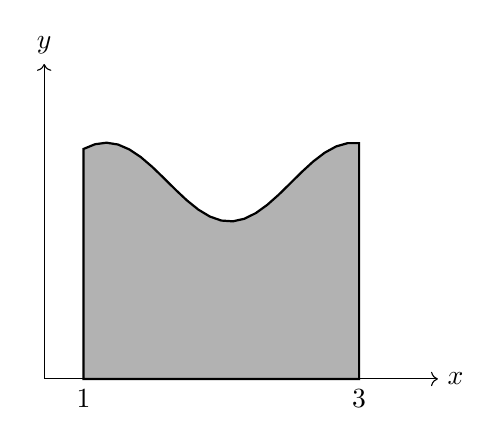
\begin{tikzpicture}[scale=0.5]
    		\draw[->] (0,0) -- (0,8) node[above] {$y$};
    		\draw[->] (0,0) -- (10,0) node[right] {$x$};

    		\filldraw[black!30,domain=1:8,variable=\x,draw=black,thick]
					(1,0) node[below,black,opacity=1] {$1$}
					-- plot (\x,{sin(\x r)+5})
					-- (8,0) node[below,black,opacity=1] {$3$}
					-- cycle;
			\end{tikzpicture}
		\end{figure}
	
		\item approximate $S_f$ by rectangle from below 13:43 JAN 6, 
			
			$j = 1, \cdots, 4$, $m_j = \inf\{f(x): x\in [x_{j-1}, x_j]\}$
			\[
				\sum_{j=1}^4 m_{j-1} (x_i-x_{j-1})\leq area(s_f)
			\]
		\item approximate $S_f$ by rectangle from above,
			$M_j = \sup\{f(x) : x\in [x_{j-1},x_j]\}$
			\[
				area \leq \sum_{j=1}^4 M_j (x_j - x_{j-1})
			\]
		\item if we can arrange lower sum $\approx$ upper sum, then we have 
			some good approximation
	\end{enumerate}

	\vspace{0.3 in}



	\subsection{Partition, Upper and Lower Sum}
	Let $a<b \in \mathbb{R}$, $f:[a,b]\in\mathbb{R}$,

	\begin{definition}[\textbf{Riemann-Darboux}]
		$ $
		
		A \textbf{partition} of $[a,b]$ is any finite set of points including
		the endpoints. 
		\[
			P:\{x_0,x_1,\cdots, x_n\} s.t. a=x_0<x_1<\cdots<x_n=b
		\]
		often for convenience, we write $P=\{a=x_0<\cdots<x_n=b\}$.
	
		A \textbf{Refinement} of $P$ is any partition $Q$ of $[a,b]$ s,t,
		$P\subseteq Q$.\\
	
		Now, fix a partition $P$ of $[a,b]$ and let $f:[a,b]\to \mathbb{R}$ be 
		bounded on $[a,b]$, i.e. $\underset{x\in [a,b]}{sup} 
		\abs{f(x)}\leq M<\infty$.	
		Write $P=\{a=x_0<\cdots<x_n=b\}$. For $j = l, \cdots, n$, 
		\begin{align*}
			m_j &= m_j(P) = \inf \{f(x) : x\in [x_{j-1},x_j]\}\\
			M_j &= M_j(P) = \sup \{f(x) : x\in [x_{j-1},x_j]\}
		\end{align*}
	Notice that $-M\leq m_k\leq M_j\leq M$ for each $j$, and these "inf", "sup"
	exist. (Using that $\mathbb{R}$ is complete.)\\
	\end{definition}

	\begin{definition}
		$ $
		\begin{itemize}
			\item \textbf{Lower Sum:}
				$L(f, P) = \sum_{j=1}^n m_j 
				\underbrace{(x_j-x_{j-1})}_{width\ of\ [x_{j-1},x_j]}$
			\item \textbf{Upper Sum:} 
				$U(f, P) = \sum_{j=1}^n M_j (x_j-x_{j-1})$\\

		\end{itemize}
	\end{definition}

	{\color{brown}
	\textbf{Remark: }
	\begin{enumerate}
		\item if $f$ is not bounded, then at least one of $L:(f,P)$ or $U(f, P)$ 
			cannot be defined. 
			
		\item we have $L(f, P)\leq U(f,P)$, Indeed, for each $j=l,\cdots, n$,
			$m_j\leq M_j$. (exactly from definition), 
			\[
				L(f, P) = \sum_{j=1}^n m_j (x_j-x_{j-1})\leq
				\sum_{j=1}^n M_j (x_j-x_{j-1}) = U(f, P)
			\]
	\end{enumerate}}

	\begin{lemma}
		If $P$ is a partition of $[a,b]$, $f:[a,b]\to \mathbb{R}$ is bounded,
		and $Q$ is a refinement of $P$, then 
		\[
			L(f,P)\leq L(f,Q) \qquad U(f,Q) \leq U(f,P)
		\]
	\end{lemma}
	\begin{proof}
		$ $
	\begin{itemize}
		\item Case 0: $Q = P$ obvious

		\item Case 1: $Q = P \cup \{q\}$ where $q\not\in P$, 

		write $ P = \{a = x_0<\cdots,x_n=b\}$ so 
		$Q = \{a=x_0<\cdots<x_{k-1}<q<x_k<\cdots<x_n=b\}$
		Then, 
		\begin{align*}
			m_k(P) &=\inf \{f(x):x\in[x_{k-1}],x_k\} 
			\qquad [x_{k-1},x_k] = [x_{k-1},q]\cup [q,x_k] \\
			&= \min\{\inf\{f(x): x\in [x_{k-1}, q]:x\in [x_{k-1},q]\}
			\inf f(x):x\in [q,x_k]\}\\
			&=\min\{m_k(Q), m_k'(Q)\} \leq m_k(Q), m_k'(Q)
		\end{align*}
		Thus, 
		\begin{align*}
			L(f,P) &=\sum_{j=1}^m m_j(P)(x_j-x_{j-1}) \\
				   &=\sum_{j=1}^{k-1} m_j(P)(x_j-x_{j-1})+m_k(P)(x_k-x_{k-1})
				   +\sum_{j=k+1}^n m_j(P)(x_j-x_{j-1}) \\
				   &\leq \sum_{j=1}^{k-1} m_j(P)(x_j-x_{j-1})+m_k
		\end{align*}
		
		\item Case 2: $Q = P\cup\{q_1, \cdots, q_m\}, q_1,\cdots,q_m$ distinct, 
		$q_u\not\in P$, by case 1, we have
		\[
			L(f,P) \leq L(f, P\cup\{q_1\})\leq L(f,P\cup\{q_1,q_2\})\leq \cdots
			\leq L(f,P\cup\{q_1,\cdots,q_m\}) = L(f,Q)
		\]
		The case $U(f,Q)\leq U(f,P)$ is similar. 
		\end{itemize}
	\end{proof}



	\begin{corollary}
		let $P, Q$ be any partition of $[a,b]$ and $f:[a,b]\to \mathbb{R}$ be 
		bounded, then 
		\[
			L(f,P)\leq U(f,Q)
		\]
	\end{corollary}
	\begin{proof}
		We have $P,Q \subseteq P\cup Q$, i.e. $P\cup Q$ refines each of $P$ and
		$Q$.
		Thus, 
		\[
			L(f,P)\leq L(f,P\cup Q) \leq U(f,P\cup Q) \leq U(f,Q) 
		\]
		
	\end{proof}






	\newpage
	\subsection{Upper and Lower Sum}

	\begin{definition}
		Given a bounded $f:[a,b]\to\mathbb{R}$, define 
		\begin{itemize}
			\item \textbf{Lower Integral} : 
				$\underline{\int}_a^b f
				= \sup \{L(f,P): P $ is a partition of $[a,b]\}$
			\item \textbf{Upper Integral:}
				$\bar{\int}_a^b f 
				= \inf \{U(f,Q): Q$ is a partition of $[a,b]\}$
		\end{itemize}
		$\underline{\int}_a^b f
		=\sup \{L(f,P): P \ is\ a\ partition \ of \ [a,b]\}
		\leq \inf \{U(f,Q): Q\ is \ a \ partition \ of \ [a,b]\} 
		=\bar{\int}_a^b f$
	
		We say that $f$ is \textbf{integrable} on $[a,b]$ provided that 
		\[
			\underline{\int}_a^b f = \bar{\int}_a^b f
		\]
		In this case, we write $\int _a^b f =  \bar{\int}_a^b f
		=\underline{\int}_a^b f$
	\end{definition}

	\underline{\textbf{Notation:}} Write 
	\[
		\int_a^b f = \int _a^b f(x)d(x) = \int_a^b f(t) dt
	\]
	
	\vspace{0.5 in}
	{\color{Brown}
	\textbf{Non-Example 1: } not every bounded function is integrable. 
		
	Define: $\chi_{\mathbb{Q}}(x) = \begin{cases}
		1, \ x\in \mathbb{Q}\\
		0, \ x\in \mathbb{R}\backslash \mathbb{Q}
	\end{cases}$.
	
	Let $P=\{0=x_0<\cdots<x_n=1\}$ be any partition of $[0,1]$, 
	We have that 
	\begin{itemize}
		\item $\mathbb{Q}$ is dense in $\mathbb{R}$, so there is 
			 $q_j\in  \mathbb{Q} \cap(x_{j-1},x_j), j = l,\cdots, n$

		\item $\mathbb{R} \backslash \mathbb{Q}$ is dense in $\mathbb{R}$, 
			so there is $r_j\in (\mathbb{R}\backslash \mathbb{Q})
			\cap(x_{j-1},x_j), j = l,\cdots, n$
	\end{itemize}
	\[
		0\leq L(\chi_{\mathbb{Q},P}) = \sum_{j=1}^n m_j(x_j-x_{j-1})\leq 
		\sum_{j=1}^n \chi_{\mathbb{Q}}(r_j)(x_j-x_{j-1})=0
		\Rightarrow \underline{\int}_0^1 = 0
	\]
	Likewise, 
	\[
		1\geq U(\chi_{\mathbb{Q}},P)\geq \sum_{j=1}^n \chi_{\mathbb{Q}}(q_j)
		(x_j-x_{j-1}) =\sum_{j=1}^n (x_j-x_{j-1}) = 1-0=1 
		\Rightarrow \bar{\int}_0^1 = 1
	\]
	hence, 
	\[
		\underline{\int}_0^1 \chi_{\mathbb{Q}} = 0 < 1
		= \bar{\int}_0^1 \chi_{\mathbb{Q}} 
	\]
	so $\chi_{\mathbb{Q}}$ is not integrable on $[0,1]$.
	}


	\newpage
	\begin{theorem}[\textbf{Cauchy Criterion For Integrability}]
		Let $a<b \in \mathbb{R}$, $f:[a,b] \to \mathbb{R}$ be bounded, then 
		TFAE,
		\begin{enumerate}
			\item $f$ is integrable on $[a,b]$
			\item given $\ep > 0$, there exists a partition $P_{\ep}$
				of $[a,b]$ s.t.  
				\[
					U(f,P_{\ep}) - L(f,P_{\ep}) < \ep
				\]
			\item given $\ep>0$, there exists a partition $P_{\ep}$ of $[a,b]$
				so for every refinement $P$ of $P_{\ep}$ 
				\[
					U(f,P) - L(f,P)<\ep
				\]
		\end{enumerate}
	\end{theorem}
	\begin{proof}
		\begin{description}
			\item 1 to 2: we assume that 
				\[
					\sup\{L(f,P): P \Par \ of \ [a,b]\}
					= \underline{\int}_a^b f = \bar{\int}_a^b 
					\inf\{U(f,P): P \Par \ of \ [a,b]\}
				\]
				Let $\ep>0$, by first equality above, there is a partition 
				$P_1$ of $[a,b]$ s.t. 
				\[
					\underline{\int}_a^b f -\frac{\ep}2<L(f,P_1)
				\]
				and by the third equality, there is a partition $P_2$ s.t.
				\[
					\bar{\int}_a^b f < U(f,P_2) - \frac{\ep}2 
				\]
				Let $P_{\ep}=P_1\cup P_2$, a refinement of $P_1$ and $P_2$,
				then since $\underline{\int}_a^b f = \bar{\int}_a^b=
				\int_a^b f$ we find   
				\[
					\int_a^b f-\frac{\ep}2 <L(f,P_1) \leq L(f,P_{\ep})\leq 
					U(f,P_{\ep}) \leq U_{f,P_2} < \int_a^b f+\frac{\ep}2
				\]
				\[
					\Rightarrow U(f,P_{\ep})-L(f,P_{\ep})<\ep
				\]
				
			\item 2 to 3: we use the lemma. 

				If $P_{\ep}\leq P$, we have 
				\[
					L(f,P_{\ep})\leq L(f,P)\leq U(f,P)\leq U(f,P_{\ep})
				\]
				Hence, 
				\[
					U(f,P_{\ep}) -L(f,P_{\ep})<\ep\Rightarrow U(f,P)-L(f,P)<\ep
				\]
			\item 3 to 2: $P_{\ep}\subseteq P_{\ep}$ i.e. $P_{\ep}$ 
				self-defines itself
			\item 2 to 1: Given $\ep>0$, there is $P_{\ep}$, a partition of
				$[a,b]$, so $U(f,P_{\ep})-L(f,P_{\ep})<\ep$.
				We have 
				\[
					L(f,P_{\ep})
					\leq \underline{\int}_a^b f
					\leq \bar{\int}_a^b f
					\leq U(f,P_{\ep}) 
					\qquad \Rightarrow \qquad 
					\underline{\int}_a^b f- \bar{\int}_a^b f < \ep
				\]
				\[
					\underline{\int}_a^b f
					= \bar{\int}_a^b f
					\qquad \Rightarrow \qquad f \ \text{is integrable}
				\]
		\end{description}
	\end{proof}

	
	
	\subsection{Continuity and Inegrability}
	\begin{definition}[\textbf{Continuous}]
		$f: I \to \mathbb{R}$ is continuous if for every $x$ in $I$, for every
		$\ep>0$, there exists $\delta >0$ s.t. for all $\abs{x-x'}<\delta$, 
		$x'\in I$, 
		\[ 
			\abs{f(x) -f(x')} < \ep 
		\]
		this definition is local. first we choose $x, \ep$, then $\delta$.\\
	\end{definition}

	\begin{definition}[\textbf{uniform Continuity}]
		$f: I \to \mathbb{R}$ is uniformly continuous if for every $\ep > 0$,
		there is $\delta > 0$ so $\abs{f(x)-f(x')}<\ep$ whenever 
		$\abs{x-x'}<\delta$ for $x, x' \in I$. \\
	\end{definition}

	\begin{proposition}[\textbf{Sequential Test of Continuity}]
		Let $f:I\to \mathbb{R}$, then $f$ is uniformly continuous $\Rightarrow$
		for any sequences $(x_n)_{n=1}^{\infty}$, $(x_n')_{n=1}^{\infty} 
		\subset I$, with $\lim_{n\to \infty} \abs{x_n-x_n'} = 0$, 
		we have $\dlim_{n\to\infty} \abs{f(x_n)-f(x_n')} = 0$. 

		[Fact $\Leftarrow$ also true]
	\end{proposition}
	\begin{proof}
		Given $\ep > 0$, let $\delta$ be as in def'n of uniform continuity.
		Since $\dlim_{n\to\infty} \abs{x_n-x_n'} =0$, there is $N\in\mathbb{N}$,
		so for $n\geq N$, we have $\abs{x_n-x_n'}<\delta$. 

		But then, for $n\geq N$, we also have that $\abs{f(x_n)-f(x_n')}<\ep$.
		i.e. $\dlim_{n\to\infty} \abs{f(x_n)-f(x_n')} = 0$.\\
	\end{proof}

	{\color{Brown}
	\textbf{Example 1}
	$f: (0,1] \to \mathbb{R}$, $f(x) = \frac 1x$. Notice that $f$ is continuous.
	
	Let $x_n=\frac 1n$, $x_n'=\frac1{2n}$, 
	$\abs{x_n-x_n'}=\frac1{2n} \overset{\to}{n\to\infty} 0$.
	\[
		\abs{f(x_n)-f(x_n')} = \abs{n-2n} = n
	:\]
	Hence, not uniformly continuous. \\

	\textbf{Example 2:} $g:(0,1]\to\mathbb{R}$, $g(x) = \sin \frac 1x$, then
	$g$ is continuous. 

	$x_n = \frac 1{\pi n}$, $x_n'=\frac 2{(2n+1)\pi}$, 
	$\abs{x_n-x_n'}=\frac1{\pi n (2n+1)} \overset{\to}{n\to\infty} 0$, 
	\[
		\abs{g(x_n)-g(x_n')} = \abs{\sin(n\pi)-\sin(\frac{2n+1}2\pi)} = 1
	\]

	For $\ep = 1$, uniform continuity fails. \\
	}

	\begin{theorem}
		Let $f:[a,b]\to \mathbb{R}$ be continuous, 
		then  $f$ is uniformly continuous. 
	\end{theorem}
	\begin{proof}
		Let us suppose that $f$ is continuous, but not uniformly continuous,
		hence there exist $\ep>0$, such that for any $\delta>0$, 
		there are $x, x' \in [a,b]$ so 
		\[
			\abs{f(x)-f(x')}\geq \ep \ while \ \abs{x-x'} < \delta
		\]
		Let us consider $\delta = \frac 1n$, so there are $x_n, x_n'$ in $[a,b]$
		such that 
		\[
			\abs{f(x_n)-f(x'_n)}\geq \ep \ while \ \abs{x-x'} < \frac 1n
		\]
		By Bolzano Weierstrass Theorem, there is a subsequence
		$(x_{n_k})_{k=1}^{\infty}$ of $(x_n)_{n=1}^{\infty}$, such that 
		$x=\dlim_{k\to\infty} x_{n_k}$ exists in $[a,b]$. 

		Then, notice that 
		\[
			\abs{x-x_{n_k}'} \leq \abs{x_n-x_{n_k}}+\abs{x_{n_k}-x_{n_k}'}
			<\abs{x-x_{n_k}}+\frac 1{n_k} 
		\]
		hence, by Squeeze Theorem, $\dlim_{k\to\infty} x_{n_k}'=x$. 
		Since $f$ is continuous, we have that 
		\[
			\lim_{k\to\infty} f(x_{n_k}) = f(x) = \lim_{k\to\infty}f(x_{n_k}')
		\]
		$\Rightarrow$
		\[
			\lim_{k\to\infty} \abs{f(x_{n_k})-f(x_{n_k}')}=0
		\]
		This contradicts that each $\abs{f(x_{n_k})-f(x_{n_k}')}\geq \ep$. 
		Thus by contradiction argument, $f'$ must be uniformly continuous. \\
	\end{proof}
	
	\begin{theorem}[\textbf{Continuous on a Closed Bounded Interval and 
		Integrability}]
		let $f:[a,b]\to\mathbb{R}$ be continuous, then $f$ is integrable. 
	\end{theorem}
	\begin{proof}
		Let $\ep>0$, then by uniform continuity of $f$, there exists a $\delta$
		such that whenever $\abs{x-x'}<\delta$, for $x, x'\in[a,b]$, 
		\[
			\abs{f(x)-f(x')} < \frac{\ep}{b-a}
		\]
		Thus, we let $P=\{a=x_0<\cdots<x_n = b\}$ be any partition with length
		$l(P) = \underset{j=1,\cdots, n}{\max} (x_{j}-x_{j-1})<\delta$.  
		
		\textcolor{Periwinkle}
		{Example: $P_n = \{a_i<a+\frac{b-a}n<a+2\frac{b-a}n
		<\cdots<a+(n-1)\frac{b-1}n<<b\}$, then $\lim_{n\to\infty} l(P_n)=0$}.

		Now, by EVT, we have 
		\begin{align*}
			x^*_j &\in [x_{j-1}, x_j] \ s.t. \ 
			f(x^*_j)=\inf\{f(x):x\in [x_{j-1},x_j]\} = m_j\\
			%
			x^{**}_j &\in [x_{j-1}, x_j] \ s.t. \ 
			f(x^{**}_j)=\sup\{f(x):x\in [x_{j-1},x_j]\} = M_j
		\end{align*}
		Then 
		\begin{align*}
			L(f,P) = \sum_{j=1}^n f(x_j^*)
			(x_j-x_{j-1})
			\qquad \qquad 
			U(f,P) = \sum_{j=1}^n f(x_j^{**})(x_j-x_{j-1})
		\end{align*}
		\begin{align*}
			U(f,P)-L(f,P)
			&= \sum_{j=1}^n (f(x^{**}_j)-f(x_j^*))(x_j-x_{j-1})\\
			&=\sum_{j=1}^n \abs{f(x_j^{**})-f(x^*_j)}(x_j-x_{j-1})
				<\sum_{j=1}^n \frac{\ep}{b-a}(x_j-x_{j-1}) \\
			&=\frac{\ep}{b-a} \cdot (b-a) =\ep
		\end{align*}
		Hence, we have satisfied the Cauchy Criterion for integrability. 
	\end{proof}

	\begin{corollary}
		if $f:[a,b]\to\mathbb{R}$ is continuous, then 
		\[
			\int_a^b f 
			= \lim_{n\to\infty} \sum_{j=1}^n f(a+j\frac{b-a}n)\frac{b-a}n 
		\]
	\end{corollary}
	\begin{proof}
		We have $a+j\frac{b-a}n \in [a+\frac{b-a}n (j-1),a+\frac{b-a}n(j-1)]$,
		$j=1,\cdots, n$. 
		
		So, 
		\[
			m_j \leq f(a+j\frac{b-a}n) \leq M_j
		\]
		and thus 
		\[
			L(f,P_n) \leq \sum_{j=1}^nf(a+j\frac{b-a}n) \frac{b-a}n \leq 
			U(f,P_n) 
		\]
		$\dlim_{n\to\infty} (U(f,P_n) - L(f,P_n)) = 0$ as 
		$\dlim_{n\to\infty} l(P_n) = 0$. 
		
		where $P_n = \{a<a+\frac{b-a}n <a+2\frac{b-a}n <\cdots<b\}$, 
		then proof of theorem shows that $\lim_{n\to\infty} L(f,P_a)
		=\int^b_a f = \lim_{n\to\infty} U(f,P_n)$ as $\lim_{n\to\infty}
		l(P_n) = \lim_{n\to\infty} \frac{b-a}n = 0$. 
 
		and hence Cauchy Criterion is satisfied, hence
		$\int_a^b f$ exists and is $\lim_{n\to\infty} L(f,P_n)$, 
		apply Squeeze Theorem. 
	\end{proof}



%------------------------------------------------------------------------------
%------------------------------------------------------------------------------
%------------------------------------------------------------------------------
%------------------------------------------------------------------------------
%------------------------------------------------------------------------------
%------------------------------------------------------------------------------
%------------------------------------------------------------------------------
%------------------------------------------------------------------------------
	\newpage
	\subsection{Basic Properties of Integrals}
	{\color{Brown}
	\textbf{Example 1: }
	We will let $a>0$ and compute $\int_0^a x^p dx$ for $p = 0, 1, 2$.
	\begin{enumerate}
		\item $p=0$, $x^p = 1$, $P = \{0 = x_0<x_1=a\}$, 
			$L(1,P) = a = U(1,P)$ 

			[$P'$ refines $P$, then $L(1,P) \leq L(l,P')\leq U(1,P') \leq 
			U(1,P) = a$]

			It follows that $\int_0^a 1 dx = a$. 
		\item From last corollary 
			\[
				\int_0^a x dx 
				= \lim_{n\to\infty} \sum_{j=1}^n (j\frac an)\frac an
				= \lim_{n\to\infty} \frac{a^2}{n^2} \sum_{j=1}^n j
				=\lim_{n\to\infty} \frac{a^2}{n^2} \frac{n(n+1)}2
				=\frac{a^2}2
			\]
		\item We need a fomula for $\sum_{j=1}^n j^2$. 

			Trick: 
			\begin{align*}
				(n+1)^3 - 1 
				&= \sum_{j=1}^n [(j-1)^3 - j^3] \tag{telescope}\\
				&= \sum_{j=1}^n [\sum_{k=0}^3 \binom{3}{k} j^k - j^3] 
				\tag{binomial theorem} \\
				&= \sum_{j=1}^n \sum_{k=0}^2 \binom{3}{k} j^k \\
				&= \sum_{k=0}^3 
			\end{align*}

			\begin{align*}
				\int_0^a x^2 dx 
				&= \lim_{n\to\infty} \sum_{j=1}^n (j\frac an)^2 \frac an\\
				&= \lim_{n\to\infty} \frac {a^3}{n^3} \sum_{j=1}^n j^2\\
				&= \lim_{n\to\infty} \frac{a^3}{3n^3} 
	a			[(n+1)^3-1-n-\frac{n(n+1)}2]\\
				&= \frac{a^3}3
			\end{align*}
	\end{enumerate}
	}

	\begin{algorithm}[\textbf{Basic Properties Of Integrals}]
			
	\end{algorithm}

	\begin{proposition}[\textbf{Additivity over intervals}]
		Let $a<b<c \in \mathbb{R}$, and $f:[a,c] \to \mathbb{R}$ satisfies
		that $f$ is integrable on each of $[a,b]$, $[b,c]$, then 
		\begin{itemize}
			\item $f$ is integrable on $[a,c]$ and  
				$\int_a^c f = \int_a^b f+\int_b^c f$.
						\end{itemize}
	\end{proposition}
	\begin{proof}
		Given $\ep > 0$, the Cauchy Criterion provides that 
		\begin{itemize}
			\item a partition $P_1$ of $[a,b]$ s.t. 
				$U(f,P_1) - L(f,P_1) < \frac{\ep}2$
			\item a partition $P_2$ of $[b,c]$ s.t. 
				$U(f,P_2) - L(f,P_2) < \frac{\ep}2$
		\end{itemize}
		Let $P$ be any refinement of $P_1\cup P_2$. Then 
		\[
			L(f,P)\geq L(f,P_1\cup P_2) = L(f,P_1) + L(f,P_2)
		\]
		\[
			U(f,P)\leq U(f,P_1\cup P_2) = U(f,P_1) + U(f,P_2)
		\]
		Then
		\[
			U(f,P)-L(f,P) \leq U(f,P_1) - L(f,P_1) +U(f,P_2) - L(f,P_2)
			<\frac{\ep}2+\frac{\ep}2 = \ep
		\]
		hence, $f$ is integrable on $[a,c]$. \\
		
		Let $P$ as above, be written $P = \{a = x_0 < \cdots < x_n = c\}$.
		
		Let $Q_1 = \{a=x_0<\cdots<x_m = b\}$, $Q_2 = \{b = x_m <\cdots<x_n=c\}$.
		
		We have 
		\[
			L(f,Q_1) \leq \int_a^b f \leq U(f,Q_1) \qquad 
			L(f,Q_2) \leq \int_b^c f \leq U(f,Q_2)
		\]
		from the proof above, we have 
		\[
			L(f,P) = L(f,Q_1)+L(f,Q_2)\leq \int_a^b f + \int_b^c f
			\leq U(f,Q_1) + U(f,Q_2) = U(f,P)
		\]
	
		Since $f$ is integrable on $[a,c]$, we have
		\[
			\int_a^c = \sup\{L(f,P):P \ partition \ of [a,c] \}
			\leq \int_a^b f + \int_a^c f \leq \inf\{U(f,P): P\ partition
			\ of [a,c]\} = \int_a^c f
		\]
		$\Rightarrow$
		\[
			\int_a^c f = \int_a^b f + \int_b^c f
		\]
	\end{proof}

%%%%%%%%%%%%%%%%%%%%%%%%%%%%%%%%%%%%%%%%%%%%%%%%%%%%%%%%%%%%%%%%%%%%%%%%%%%%%%%%
%%%%%%%%%%%%%%%%%%%%%%%%%%%%%%%%%%%%%%%%%%%%%%%%%%%%%%%%%%%%%%%%%%%%%%%%%%%%%%%%
%%%%%%%%%%%%%%%%%%%%%%%%%%%%%%%%%%%%%%%%%%%%%%%%%%%%%%%%%%%%%%%%%%%%%%%%%%%%%%%%
%%%%%%%%%%%%%%%%%%%%%%%%%%%%%%%%%%%%%%%%%%%%%%%%%%%%%%%%%%%%%%%%%%%%%%%%%%%%%%%%
%%%%%%%%%%%%%%%%%%%%%%%%%%%%%%%%%%%%%%%%%%%%%%%%%%%%%%%%%%%%%%%%%%%%%%%%%%%%%%%%

	\newpage
	\subsection{Riemann Sum - Jan 13 Mon, Jan 15 Wed}
	\begin{definition}[\textbf{Riemann Sums}]
		Let $f:[a,b]\to \mathbb{R}$, $P=\{a=x_0<\cdots<x_n=b\}$.

		A \textbf{Riemann Sum} is any sum of the following form: 
		\[
			S(f,P) = \sum_{j=1}^n f(t_j)(x_j-x_{j-1}) \qquad 
			t_j\in[x_{j-1},x_j], j = 1,\cdots, n
		\]
		
		Left Sum: 
		\[
			S_l(f,P) = \sum_{j=1}^n f(x_{j-1}) (x_j-x_{j-1})
		\]
		Right Sum: 
		\[
			S_r(f,P) = \sum_{j=1}^n f(x_{j}) (x_j-x_{j-1})
		\]
		Mid-point Sum: 
		\[
			S_m(f,P) =\sum_{j=1}^n f(\frac{x_{j-1}+x_j}2) (x_j-x_{j-1})
		\]
		Trapezoid Sum
		\begin{align*}
			T(f,P) 
			=& \frac 12 [S_l(f)+S_r(f)]\\
			=& \sum_{j=1}^n \frac{f(x_j)+f(x_j)}2 (x_j-x_{j-1})\\
			=& \frac 12 f(a)(x_1-a) +\sum_{j=1}^{n-1} f(x_j)(x_j-x_{j-1})
			+\frac 12 f(b) (b-x_{n-1})
		\end{align*}
	\end{definition}

	\begin{theorem}
		If $f:[a,b] \to \mathbb{R}$, then TFAE,
		\begin{enumerate}
			\item $f$ is integrable and 
			\item there is a number $I_f$ satisfying the following:
				given any $\ep>0$, there exists a partition $P_{\ep}$ of 
				$[a,b]$ such that 

				for any refinement of $P$ of $P_{\ep}$, any Riemann Sum of 
				$S(f,P)$ we have 
				\[
					\abs{S(f,P) - I(f)}<\ep
				\]
				Furthermore, $I_f = \int_a^b f$. 
		\end{enumerate}
	\end{theorem}
	\begin{proof}
		$ $
		
		\textbf{(i)$\Rightarrow$(ii)}
		Given $\ep>0$, the Cauchy Criterion provides that $P_{\ep}$
		so for any refinement $P$ of $P_{\ep}$, 
		\begin{equation}
			U(f,P)-L(f,P)<\ep
		\end{equation}
		Write $P = \{a=x_0<x_1<\cdots<x_n=b\}$, and let for 
		$j=1,\cdots, n$, $t_j = [x_{j-1}, x_j]$. 
		
		We observe that 
		\[
			m_j = \inf\{f(x) : x\in[x_{j-1}, x_j]\}
			\leq \sup\{f(x) : x \in [x_{j-1}, x_j]\}=M_j
		\]
		and hence 
		\[
			\sum_{j=1}^n m_j (x_j-x_{j-1}) \leq \sum_{j=1}^n f(t_j)
			(x_j-x_{j-1}) \leq \sum_{j=1}^n M_j (x_j-x_{j-1})
		\]
		i.e.
		\begin{equation}
			L(f,P) \leq S(f,P) \leq U(f,P
		\end{equation}
		Also, 
		\begin{equation}
			L(f,P) \leq \int_a^b f \leq U(f,P)
		\end{equation}
		 (1), (2) $\&$ (3) $\Rightarrow$ 
		\[
			\abs{S(f,P) - \int_a^b f} < \ep
		\]
		In particular, take $I_f = \int_a^b f$. \\

		\textbf{(ii)$\Rightarrow$(i)}
		we let for $\ep>0$, given $P_{\ep/4}$
		be a partition s.t. 
		\[
			\abs{S(f,P) - I_f} < \frac{\ep}4
		\]
		For P a refinement of $P_{\ep/4}$, $S(f,P)$ a Riemann Sum.
		We fix such $P = \{a=x_0<x_1<\cdots<x_n=b\}$. 

		For $j=1,\cdots, n$, let $m_j, M_j$ be as below, we then
		find for each $j$, 
		\[
		x_j^*, x_j^{**} \in [x_{j-1}, x_j] \qquad s.t. \qquad  
		f(x_j^*) < m_j +\frac{\ep}{4(b-a)} \qquad \& \qquad
		M_j - \frac{\ep}{4(b-a)} < f(x_j^{**})
		\]
		We then consider Riemann Sums
		\[
			S^*(f,P) = \sum_{j=1}^n f(x^*_j)(x_j-x_{j-1}), 
			\qquad S^{**}(f,P) = \sum_{j=1}^n f(x^{**}_j) (x_j-x_{j-1})
		\]
		Notice that 
		\begin{align*}
				S^*(f,P) - L(f,P) 
				&= \sum_{j=1}^n [f(x^*_j) - m_j](x_j-x_{j-1})\\
				&<\sum_{j=1}^n \frac{\ep}{4(b-a)}(x_j-x_{j-1})\\
				&= \frac{\ep}{4(b-a)} (b-a) = \frac{\ep}4
		\end{align*}
		and likewise, 
			\[
				U(f,P) -S^{**}(f,P) < \frac{\ep}4
			\]
			thus
			\begin{align*}
				&U(f,P) - L(f,P) \\
				=& U(f,P) - S^{**}(f,P) + S^{**}(f,P) - I_f
				+I_f-S^*(f,P)+S^*(f,P)-L(f,P) \\
				<& \frac{\ep}4 + \abs{S^{**}(f,P)-I_f}+\abs{I_f-S^*(f,P)}
				+\frac{\ep}4<\ep
			\end{align*}
			hence, by Cauchy's Criterion, $f$ is integrable. \\
	\end{proof}

	{\color{brown}
		\textbf{Remark:} If $f:[a,b] \to \mathbb{R}$ is continuous, then $P$ a 
	partition of $[a,b]$ then each of $L(f,P)$ and $U(f,P)$ are Riemann Sums, 
	proof: See proof of integrability of continuous. \\
	}


	\begin{proposition}[\textbf{linearity of integration}]
		Let $f,g:[a,b] \to \mR$ each be integrable and $\alpha, \beta \in \mR$,
		then 
		\begin{itemize}
			\item $\alpha f + \beta g : [a,b] \to \mR \qquad
				(\alpha f + \beta g)(x) = \alpha f(x) + \beta g(x)$
			\item $\int_a^b (\alpha f + \beta g) = \alpha \int_a^b f + \beta 
				\int_a^b g$
		\end{itemize}
	\end{proposition}
	\begin{proof}
		Let $\ep>0$, then find partitions of $[a,b]$. 
		\begin{itemize}
		\item $P_1$ s.t. for any refinement $P_p$ of $P_1$, and any Riemann Sum
			$S(f,P_p)$
			\[
				\abs{S(f,P_p) - \int_a^b f} < \frac{\ep}{2\abs{\alpha} + 1}
			\]
		\item $P_2$ s.t. for any refinement of $Q$ of $P_2$, 
			and any Riemann Sum $S(g,Q)$, 
			\[
				\abs{S(g,Q) - \int_a^b g} < \frac{\ep}{2\abs{\beta}+1}
			\]
		\end{itemize}
		Now we let $P = \{P_1\cup P_2\}$, a refinement of each of $P_1$ and 
		$P_2$, write $P=\{a=x_0<x_1<\cdots<x_n = b\}$, and choose
		$t_j \in [x_{j-1}, x_j]$ for each $j$. Then 
		\begin{align*}
			S(\alpha f +\beta g, P) 
			&= \sum_{j=1}^n (\alpha f(t_j)+\beta g(t_j)) (x_j-x_{j-1}) \\
			&=\alpha\sum_{j=1}^n f(t_j)(x_j-x_{j-1}) + 
			\beta\sum_{j=1}^n g(t_j)(x_j-x_{j-1})\\
			&= \alpha S(f,P) + \beta S(g,P)
		\end{align*}
		Then we have, 
		\begin{align*}
			\abs{S(\alpha f+\beta g, P)
				-\left[\alpha\int_a^b f+\beta\int_a^b g\right]}
			&\leq \abs{\alpha} \abs{S(f,P) - \int_a^b f} + \abs{\beta} 
			\abs{S(g,P) - \int_a^b g}\\
			&< \abs{\alpha} \frac{\ep}{2\abs{\alpha}+1} 
			+ \abs{\beta}\cdot\frac{\ep}{2\abs{\beta}+1} < \ep
		\end{align*}
	\end{proof}

	\begin{proposition}[\textbf{Order Properties of Integrals}]
		Let $f, g:[a,b]\to \mR$ each be integrable, then 
		\begin{enumerate}
			\item $f \geq 0$ $\Rightarrow$ $f \geq 0$
			\item $f \geq g \Rightarrow \int_a^b f \geq 0$
			\item $f \geq g$ on $[a,b] \Rightarrow \int_a^b f \geq \int_a^b g$
			\item $\abs{f} : [a,b] \to \mR (\abs{f}(x)= \abs{f(x)})$ 
				is integrable, with $\abs{\int_a^b f} \leq \int_a^b \abs f$
			\item $g \lor g$, $f\land g : [a,b] \to \mR$ 
				($f\lor g(x) = \max\{f(x), g(x)\} , 
				f\lor g(x) = \min \{f(x),g(x)\}$) are each integrable
		\end{enumerate}
	\end{proposition}
	\begin{proof}
		$ $
		\begin{enumerate}
			\item for any partition P, $L(f,P) > 0$. 
			\item $f - g$ is integrable with $f-g\geq 0$, 
				so $\int_a^b f - \int_a^b g = \int_a^b (f-g) \geq 0$, by 1. 
			\item let $P=\{a=x_0 <x_1 < \cdots< x_n=b\}$, and for each 
				$j=1,\cdots, n$ 
		\end{enumerate}
	\end{proof}



	
%%%%%%%%%%%%%%%%%%%%%%%%%%%%%%%%%%%%%%%%%%%%%%%%%%%%%%%%%%%%%%%%%%%%%%%%%%%%%%%%
%%%%%%%%%%%%%%%%%%%%%%%%%%%%%%%%%%%%%%%%%%%%%%%%%%%%%%%%%%%%%%%%%%%%%%%%%%%%%%%%
%%%%%%%%%%%%%%%%%%%%%%%%%%%%%%%%%%%%%%%%%%%%%%%%%%%%%%%%%%%%%%%%%%%%%%%%%%%%%%%%
%%%%%%%%%%%%%%%%%%%%%%%%%%%%%%%%%%%%%%%%%%%%%%%%%%%%%%%%%%%%%%%%%%%%%%%%%%%%%%%%
%%%%%%%%%%%%%%%%%%%%%%%%%%%%%%%%%%%%%%%%%%%%%%%%%%%%%%%%%%%%%%%%%%%%%%%%%%%%%%%
	\newpage 
	\section{ANTIDERIVATIVE}
		\subsection{Fundamental Theorem Of Calculus I - Jan 17 Friday}
	\begin{proposition}
		Let $f:[a,b]\to\mR$ be integrable on $[a,b]$, define
		\[
			F:[a,b] \to \mR, \qquad F(x) = \int_a^x f = \int_a^x f(t)dt
		\]
	\underline{Note:} no $\int_a^x f(x) dx$. 

		We may call this "integral accumulation function". 
		\begin{enumerate}
			\item $F$ is continuous on $(a,b]$
			\item $\lim_{x\to a^+} F(x) = 0$
		\end{enumerate}
		hence, we define $F(a) = 0 =\int_a^a f$. Thus $F:[a,b] \to \mR$, 
		and is continuous on $[a,b]$. 
	\end{proposition}
	\begin{proof}
		$ $
		\begin{enumerate}
			\item A1. Q5(c) assume that $f$ is integrable on each $[a,x]$, 
				$x\in [a,b]$, so $F(x) = \int_a^x f$ makes sense. Now, let 
				$a<x<x'\leq b$, and we compute 
				\begin{align*}
					F(x')-F(x) 
					&= \int_a^{x'} f - \int_a^x f\\
					&= \int_a^x f + \int_x^{x'} f -\int_a^x f 
					\tag{additivity}\\
					&= \int_x^{x'} f
				\end{align*}
				Since $f$ is integrable, it is bounded i.e. 
				$\underset{x\in [a,b]}{\sup} \abs{f(x)} = M < \infty$. 
				Thus, $\abs{f(x)} \leq M$ on $[a,b]$. Hence, by order 
				properties, 
				\[
					\abs{F(x') - F(x)} 
					= \abs{\int_x^{x'}f} \leq \int_x^{x'} \abs f
					\leq \int_x^{x'}M= M(x'-x) = M\abs{x'-x}
				\]	
				
				Thus, given $\ep>0$, let $\delta=\frac{\ep}{M+1}$, we have
				\[
					\abs{x'-x}<\delta \Rightarrow \abs{F(x')-F(x)} \leq M\delta
					=M\frac{\ep}{M+1} < \ep
				\]
				hence, $F$ is uniformly continuous on $[a,b]$. 
			\item We use $M$ as above
				\[
					\abs{\int_a^x f -0} = \abs{\int_a^x f} \leq \int_a^b\abs f
					\leq \int_a^x M = M(x-a)
				\]
				Porceed as above.\\
		\end{enumerate}
	\end{proof}

	\begin{theorem}[\textbf{Mean Value For Integrals} or \textbf{Average Value
		for Integrals}]
		Let $f:[a,b]\to\mR$ be continuous (integrability follows), then there
		exists $c\in [a,b]$, s.t. 
		\[
			\int_a^b f = f(c) (b-a)
		\]
	\end{theorem}
	\begin{proof}
		We use two important facts about continuous functions. 
		
		By \textbf{EVT}, there exists $x^*, x^{**} \in [a,b]$ s.t.
		\[
			f(x^*) = m = min \{f(x) : x\in [a,b]\} \qquad and \qquad
			f(x^**) = M \max\{f(x) : x \in [a,b]\} 
		\]
		Then $m\leq f\leq M$, on $[a,b]$ so order properties provide
		\[
			m(b-a) =\int_a^b m\leq \int_a^b f \leq \int_a^b M = M(b-a)
		\]
		so 
		\[
			f(x^*) = m\leq \frac1{b-a} \int_a^b f \leq M = f(x^{**})
		\]
		By \textbf{IVT}, Since $f(x^*) \leq \frac1{b-a}\int_a^b f
		\leq f(x^{**})$, there is $c$ between $x^*$ and $x^{**}$, and 
		hence $c\in[a,b]$ s.t. 
		\[
			f(c) = \frac1{b-a} \int_a^b f
		\]
	\end{proof}

	{\color{brown}
	\textbf{Remark:}
	$f$ is integrable $\Rightarrow$ $F(x) = \int_a^b f$ is a cts function. 
	$f$ cts $\Rightarrow$ $F$ differentiable. (BELOW) }\\
		
	\begin{theorem}[\textbf{Fundamental Theorem of Calculus (I)}]
		Let $f:[a,b]\to \mR$ be \underline{continuous}, then 
		\[
			F:[a,b] \to \mR, \qquad F(x) = \int_a^x f
		\]
		satisfies that $F$ is differentiable on $[a,b]$, with $F' = f$ 
		on $[a,b]$.
	\end{theorem}
	\begin{proof}
		Let $x\in[a,b]$, we want to examine the quotient 
		\[
			\frac{F(x+h)-F(x)}h \qquad when \qquad x+h \in [a,b]
		\]
		\underline{$h>0$}, 
		\[
			\frac{F(x+h)-F(x)}h=\frac 1h \cdot \int_x^{x+h} f = 
			\frac1h \cdot f(c_h^*) (x+h-x)=f(c_h^*) 
		\]
		by M.V.T for I, where $c_h^* \in [x, x+h]$, 

		\underline{$h<0$}, 
		\[
			\frac{F(x+h)-F(x)}h = \frac{F(x)-F(x+h)}{-h}
			= \frac1{-h} \cdot \int_{x+h}^x f
			= \frac1{-h}\cdot  f(c_h^{**})(x-(x+h))
			=f(c_h^{**})
		\]
		by M.V.T for I, where $c_h^{**} \in [x + h, x]$. 
			
		hence, 
		\[
			\lim_{h\to 0} \frac{F(x+h)-F(x)}h 
			=\underbrace{\lim_{h\to 0} f(c_h^*)}_{continuity}	
			=\underbrace{\lim_{h\to 0} f(c_h^{**})}_{squeeze}= f(x)
		\]
		Thus, $F'(x)$ exists, and equals $f(x)$, for $x\in [a,b]$. \\
		
		{\color{brown}
		\textbf{Remark:} Notice that we really found 
		\begin{itemize}
			\item left derivative at $x=b$
			\item right derivative at $x=a$
		\end{itemize}}
	\end{proof}

	\begin{notation}
		Let $-\infty \leq a < b \leq \infty \in \mR$, $f:[a,b] \to \mR$ be 
		continuous, fix $c \in (a,b)$, dfeine 
		\[
			F:(a,b) \to \mR, F(x) = 
			\begin{dcases}
				\int_c^x f, & x \geq c\\
				-\int_x^c f, & x < c
			\end{dcases}
		\]
		We know from FToCI, that $F'(x) = f(x)$ for $x > c$. \\
	\end{notation}

	\begin{proposition}
		Let us compute $F'(x)$ for $x < c$, let $c'\in (a,c)$ and for $x \in 
		(c',c)$ we have 
		\begin{alignat*}{2}
			& &\qquad \int_{c'}^c f &= \int_{c'}^x f + \int_x^c f \\
			\Rightarrow& &\qquad 
			-\int_x^c f &= \int_{c'}^x f - \int_{c'}^c f \\
			\Rightarrow& &\qquad 
			F'(x) &= \frac{d}{dx} \int_{c'}^x f - \int_{c'}^c f =f(x)
		\end{alignat*}
		It will be convecient, hereafter, to let $\int_c^x f = - \int_x^c f$
		if $x <c$, and we have FToCI
		\[
			\frac d{dx} \int_c^x f = f(x), \qquad x \in (a,b).
		\]
	\end{proposition}
	


	\newpage
	\subsection{Logrithm and Exponential Functions}

	\begin{definition}
		For $x \in (0,\infty)$, 
		\[
			L(x) = \int_1^x \frac 1t dt
		\]
		we shall use only integral $\&$ differentiation rates to gain theory of
		$L$. \\
	\end{definition}
		
	\begin{proposition}
		If $a,b > 0$, gthen $L(ab) = L(a)+L(b)$.
	\end{proposition}
	\begin{proof}
		Let $F(x) = L(ax)$, then chain rule provides 
		\[
			F'(x) = \frac1{ax} \frac d{dx}(ax) = \frac 1x =L'(x)
		\]
		hence, $F' - L' = 0 \Rightarrow F-L=C$ (constant), by MVT, 
		$F = L+C (*)$.
		Then, 
		\[
			L(a) = F(1) = L(1) + C = C. 
		\]
		Also, $L(ab) = F(b) = L(b) + L(a)$. \\
	\end{proof}

	\begin{proposition}
		For $a > 0$, $q \in \mQ$, $L(a^q) = qL(a)$, (convention: $a^0=1$).
	\end{proposition}
	\begin{proof}
		First: $n \in \mN$, 
		\setcounter{equation}{0}
		\begin{equation}
			L(a^n) = L(a)+L(a^{n-1}) = \cdots = 
			\underbrace{L(a) + L(a)
			+ \cdots + L(a)}_{n} = nL(a)
		\end{equation}
		
		Second: 
		\begin{equation}
			L(a) = L((a^{\frac1n})^n) = nL(a^{\frac1n}) 
			\Rightarrow L(a^{\frac1n})=\frac1n L(a)
		\end{equation}
		
		Third: 
		\begin{equation}
			0 = L(1) = L(aa^{-1})=L(a)+L(a^{-1})\Rightarrow L(a^{-1})-L(a)
		\end{equation}
		
		Then, (1) $\&$ (2) $\Rightarrow$ $L(a^m) = mL(a)$, for $m \in \mZ$,
		for $q = \frac mn$, $m \in \mZ$, $n\in \mN$. 

		We combine (1), (2), $\&$, (3) to get $L(a^q) = mL(a^{\frac1n})
		=\frac mn L(a)$.\\
	\end{proof}
	
	
	\begin{proposition}
	$ $
		\begin{enumerate}
			\item L is inreasing: $0<x<x'$ then $L(x) < L(x')$ 
			\item $\lim_{x\to 0^+} L(x) = -\infty$, $\lim_{x\to\infty} L(x) 
				=\infty$
		\end{enumerate}
	\end{proposition}
	\begin{proof}
		 $ $
		\begin{enumerate}
			\item 
				\[
					L(x') - L(x) = \int_x^{x'} \frac 1t dt \geq \int_x^{x'}
					\frac1{x'} dt = \frac1{x'}(x'-x) > 0
				\]
				Alternatively: $L'(x) = \frac1x>0$, MVT $\Rightarrow L$ is 
				strictly increasing. 
			
			\item To see that $\lim_{x\to\infty} L(x) = \infty$, it suffices
				to find $(a_n)_{n=0}^{\infty} \subset (0,\infty)$ 
				s.t. $\lim_{n\to\infty} a_n = \infty$ and $\lim_{n\to\infty}
				L(x_n) = \infty$. 
				Consider $(2^n)_{n=0}^{\infty}$ and we have $\lim_{n\to\infty}
				L(2^n) = \lim_{n\to\infty} nL(2) = \infty$. Likewise, 
				$\lim_{n\to\infty} 2^{-n}=0$, and $\lim_{n\to\infty}(2^{-n})
				=\lim_{n\to\infty} (-n)L(2) = -\infty$. 
		 \end{enumerate}

	\end{proof}

	\begin{corollary}
		$L:(0,\infty) \to \mR$ is one-to-one and onto. 
	\end{corollary}
	\begin{proof}
		Increasing $\Rightarrow$ one-to-one, since $\lim_{x\to 0^+} = -\infty$,
		$\lim_{x\to\infty} L(x) = \infty$, and IVT provides that $L$ is onto.\\
	\end{proof}
	
	\begin{definition}
		$E: \mR \to (0,\infty)$ to be $L^{-1}$: inverse function. Hence,
		\[
			E(L(x)) = x, x\in (0,\infty) \qquad and \qquad 
			L(E(y)) = y \qquad if \ y \in \mR
		\]\\
	\end{definition}
	
	\begin{proposition}
		If $y \in \mR$, $L(E(y)) = y$, 
		$\underset{\Rightarrow}{chain \ rule} \frac1{E(y)} E'(y) = 1$\\
		$\Rightarrow E'(y) = E(y)$\\
	\end{proposition}
	
	\begin{algorithm}[\textbf{About $E$}]
		Let $c,d \in \mR$, 
		\begin{enumerate}
			\item $E(c+d) = E(c) E(d)$
			\item $E(-c) = \frac1{E(c)}$
			\item $E(0)=1$
			\item $E(qc) = E(c)^q$, $q \in \mQ$ 
		\end{enumerate}
	\end{algorithm}
	\begin{proof}
		\begin{enumerate}
			\item Let $c=L(a)$, $d = L(b)$ (L is onto)
				$E(c+d) = E(L(a) + L(b)) = E(L(ab)) = ab = E(a)E(b)$
			\item $L(1) = 0$ so $E(0)=1$
			\item use (1) and (2)
			\item $E(qc) = E(qL(a)) = E(L(a^q)) = a^q = E(c)^q$. 
		\end{enumerate}
		
	\end{proof}

	\textbf{What is $E(1)$?} We note that 
	\[
		\lim_{h\to 0} \frac{L(1+h)}{h} = L'(1) = \frac11=1
	\]
	Hence,
	\[
		1 = \lim_{n\to\infty} \frac{L(1+\frac1n)}{\frac1n} 
		=\lim_{n\to\infty} n L(1+\frac1n) = \lim_{n\to\infty} L((1+\frac1n)^n)
	\]
	Since $E$ is continuous, 
	\[
		E(1) = E(\lim_{n\to\infty}L((1+\frac1n)^n)) = \lim_{n\to\infty}
		E(L((1+\frac1n)^n)) = \lim_{n\to\infty} (1+\frac1n)^n = e
	\]

	From rule (iv), $E(q) = e^q$ for $q \in \mQ$, 
	if $x \in \mR$, write $x = \lim_{n\to\infty} q_n$, each $q_n \in \mQ$, 
	and we define 
	\[
		e^x = E(x) = \lim_{n\to\infty} E(q_n) = \lim_{n\to\infty} e^{q_n}
	\]

	\begin{definition}
		For $a>0$, we have $a = E(L(a)) = e^{L(a)}$, and we let
		\[
			a^x = E(L(a)x) = e^{L(a) x}
		\]
	\end{definition}

	\textbf{Exercise With Chain Rule: }
	\begin{enumerate}
		\item $\frac d{dx} (a^x) = L(a)a^x$, 
		\item $L(a^x) = L(a) x = xL(a)$,
		\item $p\in\mR$, $x>0$, $x^p = e^{p(L(x))}$, 
			$\frac d{dx} (x^p) = px^{p-1}$
	\end{enumerate}



	
	\newpage
	\subsection{Fundamental Theorem of Calculus II - Jan 22}
	
	\begin{theorem}[\textbf{Fundamental Theorem of Calculus II}]
		Let $f, F : [a,b] \to \mR$ satisfy that 
		\begin{itemize}
			\item $f$ is integrable
			\item $F$ is continuous on $[a,b]$ 
			\item $F$ is differentiable on $(a,b)$, with $F' = f$ on $(a,b)$
		\end{itemize}
		Then, 
		\[
			F(b) - F(a) = \int_a^b f
		\]
	\end{theorem}
	\begin{proof}
		Let $\ep>0$, find a partition $P_{\ep}$ on $[a,b]$, so 
		\begin{itemize}
			\item for every refinement $P$ of $P_{\ep}$
			\item for every Riemann Sum $S(f,P)$, we have 
				\[
					\abs{S(f,P) - \int_a^b f} < \ep
				\]
		\end{itemize}
		Take $P$ as above, write $P=\{a = x_0 < x_1 < \cdots < x_n = b\}$. 

		Now let us consider $F$ on each $[x_{j-1}, x_j]$ 
		\begin{itemize}
			\item $F$ is continuous on $[x_{j-1}, x_j]$
			\item $F$ is differentiable on $[x_{j-1}, x_j]$ [can be used in 
				closed interval, except for $j=0,n$]
		\end{itemize}
		Thus MVT tells us there exists $c_j\in(x_{j-1}, x_j) \subset [x_{j-1},
		x_j]$ such that 
		\[
			F(x_j)-F(x_{j-1}) = F'(c_j) (x_j-x_{j-1})
			=f(c_j) (x_j-x_{j-1}) \qquad (*)
		\]
		Now we consider
		\begin{align*}
			F(b) - F(a) 
			=& \sum_{j=1}^n [F(x_j) - F(x_{j-1})] \tag{telescope}\\
			=& \sum_{j=1}^n f(c_j) (x_j-x_{j-1}) \tag{by *}\\
			=& S(f,P) \tag{a Riemann Sum} 
		\end{align*}
		Hence, 
		\[
			\abs{F(b) - F(a) - \int_a^b f} = \abs{S(f,P) - \int_a^b f} < \ep
		\]
		
		Since $\ep>0$ is arbitrary, we get desired result. 
	\end{proof}

	{\color{brown}
	\textbf{Remark:}
	\begin{itemize}
		\item Suppose $F, G : [a,b] \to \mR$, both satisfy $F' = f =
	G'$, for integrable $f$, then 
	\[
		(F-G)' = F'-G' = f-f = 0 
		\underset{\Rightarrow}{M.V.T} F - G = C (constant)
	\]
	hence, $F(x) = G(x) + C$ for any $x$ in $[a,b]$. 
	
	\item 
		If $f:[a,b]\to \mR$ is continuous, then $f$ is integrable
		(theorem from earlier) $\&$ $F(x) = \int_a^b f$ defines on 
		antiderivative.

		Moral: $f$ continuous $\to$ an antiderivative exists. \\
	\end{itemize}
	}


	\begin{notation}
		If $f$ is continuous, (on same intervals), and $F$ is an antiderivative
		of $f$, i.e. $F' = f$ (on interval of said intervals), write 
		$\int f(x) dx = F(x) + C$.\\
	\end{notation}
	
	\textbf{Antiderivatives of Basic Functions: }
	\begin{align*}
		p\neq -1, \qquad \int x^p dx &= \frac{x^{p+1}}{p+1} + C & 
		\int e^x dx &= e^x + C & & \\
		\int \cos x dx &= \sin x + C
			& \int \sin x dx &= -\cos x + C\\
		\int \sec^2 x dx& = \tan x + C & \int \sec^2 x dx &= \tan x + C
	\end{align*}
	\begin{align*}
		\int \frac1{x^2+1}dx 
		= \arctan x + C
		[Tan = \tan\rvert_{(\frac{\pi}2, \frac{-\pi}2)]
			: (-\frac{\pi}2 , \frac{\pi}2)\to \mR}  \qquad 
			\text{one-to-one and onto}\\
		%
		\int \frac1{\sqrt{1-x^2}}dx 
		= \arcsin x + C
		[\Sin = \sin\rvert_{(\frac{\pi}2, \frac{-\pi}2)]
		: (-\frac{\pi}2, \frac{\pi}2)\to [-1,1]}  \qquad 
			\text{one-to-one and onto}\\
	\end{align*}
	
		\begin{theorem}[\textbf{Change of Variables/Substitution/Reverse
		Chain Rule}]
		Suppose 
		\begin{itemize}
			\item $g:[a,b] \to \mR$, differentiable with $g'$ continuous
			\item $f$ is defined on $g([a,b])$ with $f \circ g : [a,b]
				\to \mR$ continuous
		\end{itemize}
		Then 
		\[
			\int_a^b f(g(x)) g'(x) dx = \int_{g(a)}^{g(b)} f(u)d(u)
		\]
		Anti Derivative Form:
		\[
			\int f(g(x)) g'(x) dx = \int f(u)du \vert_{u=g(x)}
		\]
	\end{theorem}
	\begin{proof}
		Let $F$ be any antiderivative of $f[g[(a,b)]=[c,d],$ let 
		$F(x) = \int_x^c f]$. 
		
		Let $H:[a,b] \to \mR$ be given by $H(x) = F(g(x))$. 
		Then Chain Rule provides 
		\[
			H'(x) = F/(g(x))g'(x) = f(a(x))g'(x)
		\]
		and F.T. of C II provides that 
		\[
			H(b) - H(a) = \int_a^b f(g(x))g'(x) dx
		\]
		but F.T.of C provides that 
		\[
			\int_{g(a)}^{g(b)} f(u)d(u) = F(g(b)) - F(g(a)) = H(b) - H(a)
		\]
	\end{proof}

	{\color{Brown}
	\textbf{Example: }
	\begin{enumerate}
		\item 
			\begin{align*}
			\int xe^{-x^2} dx 
			&= -\frac12 \int e^{-x^2} (-2x) dx\\
			&= -\frac12 \int e^u du \\
			&= -\frac12 e^u + C \\
			&= -\frac12 e^{-x^2} + C
			\end{align*}
			
		\item 
			\begin{align*}
				\int_1^3 x(x^2+4)^{91} dx
				&= \frac 12 \int_5^{13} u^{91} dx\\
				&= \frac 12 \frac{u^{92}}{92} \vert^{13}_5 \\
				&= \frac1{184} [(13)^{92}-5^{92}]
			\end{align*}

		\item 
			\begin{align*}
				\int \cos^m x \sin^n x dx \tag{n \ odd}
				&= \int \cos^m x \sin^{2k} x \sin x dx\\
				&= \int \cos^m x(1-\cos^2 x)^k \sin x dx
				\tag{$ u = \cos x, \  du = -\sin x dx$}\\
				&= -\int u^m(1-u^2)^k du \vert_{u=\cos x}
			\end{align*}
	\end{enumerate}}
%------------------------------------------------------------------------------
%------------------------------------------------------------------------------
%------------------------------------------------------------------------------
%------------------------------------------------------------------------------
%------------------------------------------------------------------------------
%------------------------------------------------------------------------------
%------------------------------------------------------------------------------

\newpage
\subsection{Integration and Trignometry - Jan 22 Wed, TUT}
\begin{definition}
	$\pi = 2\int_{-1}^a \sqrt{a-x^2}dx$ \\
\end{definition}

\begin{definition}
	Let for $-1\leq x\leq 1$, 
	\[
		\arccos x = x \sqrt{1-x^2} + 2\int_x^1 \sqrt{1-u^2} du
	\]
	Then $\frac12 \arccos x$ is the area of 
	-----graph-----
\end{definition}

\textbf{Note:} $\frac12\arccos x$ is proportional to the angle $\theta$,
hence it is reasonable to measure. 
\[
	\theta = \arccos x \qquad "radians"
\]
\begin{itemize}
	\item $\arccos -1 = \pi$
	\item $\arccos 0 = 2\int_0^1 \sqrt{1-u^2} du \overset{symmetry}{=}
		\int_{-1}^1 \sqrt{1-u^2} du = \frac{\pi}2$
	\item $\arccos 1 = 0$
\end{itemize}

\textbf{Derivatives:}
\begin{align*}
	\arccos ' x 
	&= \sqrt{1-x^2} + x\frac12(1-x^2)^{-\frac 12} (-2x) - 2\sqrt{1-x^2}\\
	&= -\frac{x^2}{\sqrt{1-x^2}}-\sqrt{1-x^2}\frac{\sqrt{1-x^2}}
		{\sqrt{1-x^2}} = -\frac{1}{\sqrt{1-x^2}}
\end{align*}
hence, 
\begin{itemize}
	\item $\arccos 'x < 0$ and by MVY, decreasing
	\item $\lim_{x\to -1^+} \arccos 'x = -\infty = \lim_{x\to 1^-}
		\arccos 'x$ 
	\item $\arccos '0=-1$
	\item $\arccos ''(x) = -\frac x{(1-x^2)^{\frac 32}}$ hence, \\
		- $\arccos ''(x) > 0$ if $x <0  \Rightarrow $ concave up\\
		- $\arccos ''(x) <0$ if $x > 0 \Rightarrow$ concave down\\
\end{itemize}

\begin{definition}
	$ $
	\begin{itemize}
		\item $\Cos x = \arccos ^{-1} : [0,\pi] \to [-1,1]$

		\item $\sin \theta = \sqrt{1-\cos^2 \theta}$
	\end{itemize}
			
	Hence, $\sin:[0,\pi] \to [0,1]$, with 
	\begin{itemize}
		\item $\Sin(0) = \sqrt{1-1^2} = 0$
		\item $\Sin(\frac{\pi}2) = \sqrt{1-0^2} = 0$
		\item $\Sin(\pi) = \sqrt{1-(-1)^2} = 0$
	\end{itemize}
\end{definition}

\textbf{Derivatives of $\cos$, $\sin$}

$\arccos (\cos \theta) = \theta$
\[
	\underset{\text{Chain Rule}} {\Rightarrow}
	\frac{-1}{\sqrt{1-\cos^2 \theta}} \cos '\theta=1
	\Rightarrow \cos'\theta = -\sin \theta
\]

\[
	\sin'\theta = \frac d{d\theta} \sqrt{1-\cos^2\theta} 
	= \frac1x(1-\cos^2 \theta) ^{-\frac12} (-2\cos \theta \cos'\theta)
	= \cos \theta
\]
Hence, $\sin'(0)=1$, $\sin'\frac{\pi}2 = 0$, $\sin'(\pi) = -1$, and 
$\sin"(\theta) = -\sin \theta < 0$ if $0<\theta < \pi \Rightarrow$
concave down

\underline{Extension to $\mR$} 
\begin{enumerate}[label=(\alph*)]
	\item we define $\cos, \sin:[-\pi,\pi] \to [-1,1]$
		\begin{itemize}
			\item $\cos$ is even: $\cos (-\theta) = \cos \theta$,
			$\theta \geq 0$
			\item $\sin$ is odd: $\sin(-\theta) = -\sin \theta$, 
				$\sin \theta = \Sin x$, if $\theta \geq 0$ 
		\end{itemize}
	\item we define $\cos, \sin : \mR \to [-1, 1]$
		\[
			\cos(\theta + 2\pi n) = \cos(\theta)
			\qquad 
			\sin (\theta + 2\pi n) = \sin(\theta)
			\qquad 
			\theta \in [-\pi, \pi], n \in \mZ
		\]
\end{enumerate}

\begin{lemma}
	Let $f: \mR \to \mR$ is twice differentiable, then 
	\begin{itemize}
		\item $f(0) = f'(0) = 0$ and 
		\item $f''+f=0$
	\end{itemize}
	then $f=0$. 
\end{lemma}
\begin{proof}
	Let $g=(f')^2 + f^2$ then
	\[
		g(0)=0 \qquad and \qquad 
		g'= 2ff'+ 2ff'=2f[f''+f] = 0
	\]
	$\Rightarrow$ by MVT, $g$ constant, hence, $g=0$, 
	then $0\leq f^2 \leq g$. 
\end{proof}

\begin{lemma}
	Double Angle Fomula for Cos
\end{lemma}
\begin{proof}
	Let $a, b \in \mR$ be fixed, defined $f : \mR \to \mR$, 
	\[
		f(t) = \cos(s+t) - a \sin t + b\cos t
	\]
	Then
	\begin{align*}
		f'(t) & = - \sin (s+t) + a\sin t + b \cos t\\
		f''(t) &= -\cos (s+t) + a\cos t -b\sin t\\
		\Rightarrow f''+f &= 0
	\end{align*}
	Now we wish to choose $a$, $b$ to satisfy
	
	$f(0)=0$, hence $0=f(0)=\cos s - a \Rightarrow a = \cos s$\\
	$f(0)=0$, hence $0=f'(0)=-\sin s + b \Rightarrow b = \sin s$

	With these choices of $a,b$, the lamma tells us that $f(t) = 0$, hence
	\[
		0 = \cos(s+t) - [\cos s \cos t-\sin s \sin t)
	\]
\end{proof}

\textbf{Double Angle Fomula for $\cos$: }
Since $\cos^2 t + \sin^2 t = 1$, the angle sum fomula gives
\[
	\cos 2t = \cos^2 t - \sin^2 t = 
	\begin{cases}
		1 - 2\sin^2 t \Rightarrow\sin^2 t = \frac12[1-\cos^2 t]\\
		2\cos^2 t - 1 \Rightarrow \cos^2 t = \frac12 [1-\cos^2 t]
	\end{cases}
\]

\begin{lemma}
	Double Angle Fomula for $\sin$: $\sin(s+t) = \cos s \sin t + \sin x
	\cos t$
\end{lemma}
\begin{proof}
	Fix $s \in \mR$, for $t$ consider
	\[
		\cos (s + t) = \cos s \cos t - \sin s \sin t
	\]
	and take $\frac d{dt}$ to both sides.
\end{proof}

\textbf{Double Angle Fomula for $\sin$: }
\[
	\sin 2t = 2\cos t \sin t
\]

{\color{Brown}
	\textbf{Example 1:}
	\begin{enumerate}
	\item 
		\begin{align*}
			\int \sin^2x dx
			=& \frac12 \int(1-\cos 2x) dx\\
			=& \frac12 [x-\frac12 \sin 2x] + C\\
			=& \frac12 x - \frac 14 \sin 2x + C\\
			=& \frac12 x - \frac12 \sin x \cos x + C
		\end{align*}

	\item
		\begin{align*}
			\int \cos^4 x dx 
			=& \int[\frac12(1+\cos 2x)]^2 dx\\
			=& \frac 14 \int (1+ 2\cos 2x + \cos^2 2x) dx\\
			=& \frac 14 \int (1+2\cos 2x + \frac12[1+\cos4x]) dx
		\end{align*}

	\item 
		\begin{align*}
			&\int \sin x \cos^4 x dx \tag{$u = \cos x, du = -\sin xdx$}\\
			=& - \int u^4 du\vert_{u=\cos x} \\
			=& -\frac{\cos^5 x}5 + C
		\end{align*}
		
	\item
		\begin{align*}
			\int \sin^2x \cos^4 x dx
			=& \int \sin^2x\cos^2x\cos^2xdx\\
			=& \int (\frac12\sin2x)^2 \frac12[1+\cos 2x]dx\\
			=& \frac 18 \int[\sin^22x + \sin^22x\cos 2x] dx
		\end{align*}
	\end{enumerate}
}

\textbf{Change of Variables(Antiderivatives form)}
\[
\int f(g(x))g'(x)dx = \int f(u) du \vert_{u=g(x)}
\]
$f, g'$ continuous.

\textbf{Inverse Form: }Suppose we try $x = g(u)$, 
\[
	\int f(x) dx = \int f(g(u))g'(u) du\vert_{x=g(u)}
\]

\begin{algorithm}[\textbf{Trig Substitution}]
	$ $
	\begin{center}
	\begin{tabular}{c c c c}
		Forms &  Substitution & Main Identity & $dx$ \\
		$a^2-x^2$ & $x = a\sin \theta$ & $a^2 - x^2 = a^2 \cos ^2 \theta$
				  & $dx = a\cos \theta d\theta$\\
		$x^2+a^2$ & $x = a\tan \theta$ & $x^2+a^2=a^2\sec\theta$
				  & $dx = a\sec^2\theta d\theta$
	\end{tabular}
	\end{center}
\end{algorithm}

{\color{Brown}
\textbf{Examples}
\begin{enumerate}
	\item 
		\begin{align*}
			\int \frac{dx}{(9-x^2)^{3/2}}
			=&\int \frac{3\cos \theta}{(9\cos^2\theta)^{3/2}}dx\\
			=&\frac 19 \int \sec^2\theta d\theta 
			= \frac 19 \tan \theta + C \\
			=& \frac 19 \frac{\sin\theta}{\sqrt{1-\sin^2\theta}}+C\\
			=& \frac 19 \frac{\frac13 x}{\sqrt{1-(\frac13x)^2}}+C
			= \frac 19 \frac x{\sqrt{9-x^2}}+C
		\end{align*}
	\item 
		\begin{align*}
			\int \frac{dx}{x^2+2x+5} 
			&= \int \frac{dx}{(x+1)^2+4} 
			\tag{$x+1=2\tan\theta, dx=2\sec^2\theta d\theta$}\\
			&= \int \frac{2\sec^2\theta}{2^2\sec^2\theta}d\theta\\
			&= \frac12 \int d\theta = \frac12 \theta+C\\
			&= \frac12 \arctan \frac{x+1}2 + C
		\end{align*}

	\item 
		\begin{align*}
			\int \sqrt{1-x^2}dx
			=& \int \cos^2\theta d\theta\\
			=& \frac 12 \int [1+\cos 2\theta]d\theta\\
			=& \frac12[\theta + \frac12 \sin 2\theta] + C\\
			=& \frac12[\arcsin x + \sin \theta \cos \theta] + C\\
			=& \frac 12[\arcsin x]+ x\sqrt{1-x^2} + C\\
			\Rightarrow &\arcsin (x) = 2\int\sqrt{1-x^2}dx -x\sqrt{1-x^2}
			+ C'\\
			[\arcsin x &= \frac{\pi}2 -\arccos x] \checkmark
		\end{align*}

	\item 
		\begin{align*}
			\int \frac{dx}{\sqrt{x^2+1}}\tag{$x = \tan \theta, 
			dx = \sec^2 \theta d\theta$}
			=& \int \frac{\sec^2 \theta d\theta}{\sec \theta}\\
			=& \int \sec \theta d\theta\\
			=& \int \sec\theta \frac{\sec \theta \tan \theta}
			{\sec\theta + \tan \theta} d\theta\\
			=& \int \frac{\sec^2\theta +\tan \theta \sec \theta}
			{\sec \theta + \tan \theta} d\theta\\
			=& \log \abs{\sec\theta + \tan \theta} + C\\
			=& \log (\sqrt{x^2+1}+x)+C
		\end{align*}

	\item 
		\begin{align*}
			\int \frac{dx}{\sqrt{x^2+1}}\tag{$x = \tan \theta, $}
			=& \int \frac{\cosh t}{\cosh t} dt
		\end{align*}
\end{enumerate}

}

%------------------------------------------------------------------------------
%------------------------------------------------------------------------------
%------------------------------------------------------------------------------
%------------------------------------------------------------------------------
%------------------------------------------------------------------------------
%------------------------------------------------------------------------------
%------------------------------------------------------------------------------

\newpage
\subsection{Integration by Partial Fraction - Jan 27}

\textbf{Warm Up: }

\begin{align*}
	\int \sec\theta d\theta 
	=& \int \frac1{\cos\theta} d\theta\\
	=& \int \frac{\sin^2\theta + \cos^2\theta}{\cos \theta} d\theta\\
	=& \int\frac{\sin^2\theta}{\cos\theta} d\theta+\int\cos\theta d\theta\\
	=& \int \frac{\sin^2\theta}{1-\sin^2\theta}\cos\theta d\theta 
	+ \int \cos\theta d\theta \\
\end{align*}

\begin{theorem}
	$ $
	\begin{enumerate}
	\item 
	Let $q\neq 0$ be a polynomial with $\mR$-coefficients, then 
	we may write 
	\[
		q(x) = a(x-r_1)^{m_1} \cdots (x-r_m)^{m_m}\cdot
		(x^2+b_1x+c_a)^{n_1} \cdots (x^2 + b_Nx + C_N)^{n_N}
	\]
	where $a\neq 0$, $r_1, \cdots, r_M$ are the distinct $\mR$-roots
	 of $q$, and $b_1, \cdots, b_N, \cdots, c_N \in \mR$.. 

	 $b_j^2 - 4c_j < 0$ for $j=1, \cdots, N$. Also, $m_1, \cdots, m_N,
	 n_1, \cdots, n_N \in \mN$. 
	 
	\item 
	Let $p$ be $\mR-$polynomial with 
	\[
		\deg p < \deg q
	\]
	Then there are unique $\mR-$numbers $A_1, \cdots, B_N, C_N$. 
	so 
	\[
	\frac{p(x)}{q(x)} = \sum_{j=1}^M \sum_{k=1}^M \frac{A_j,k}{(x-{r_j})^k}
	= + \sum_{j=1}^N\sum_{k=1}^{n_j} \frac{B_{j,k}x + C_{j,k}}
	{x^2+b_jx+c_j}^k
\]
	\end{enumerate}
\end{theorem}





%------------------------------------------------------------------------------
%------------------------------------------------------------------------------
%------------------------------------------------------------------------------
%------------------------------------------------------------------------------
%------------------------------------------------------------------------------
%------------------------------------------------------------------------------
%------------------------------------------------------------------------------

\newpage
\subsection{Integration by parts - Jan 29}
\begin{theorem}[\textbf{Integration by Parts/"Reverse Product Rule"}]
	Let $f, g F:[a,b] \to \mR$ satisfy
	\begin{itemize}
		\item $f$ is integrable on $[a,b]$
		\item $F' = f$ on $[a,b]$
		\item $g'$ is integrable on $[a,b]$
	\end{itemize}
	Then 
	\[
		\int_a^b f(x)g(x)dx = F(b)g(b) - F(a)g(a) - \int_a^b F(x)g'(x)dx
	\]
	\textbf{Antiderivative Form: }
	\begin{align*}
		\int f(x)g(x)dx &= F(x)g(x) - \int F(x)g'(x)dx, \qquad 
			F(x) = \int f(x)dx \qquad \text{Can choose $c=0$}\\
		\int f'g &= fg-\int fg'
	\end{align*}
\end{theorem}
\begin{proof}
	Product Rule: 
	\[
		\frac{d}{dx} [F(x)g(x)] = F'(x)g(x) + F(x)g'(x)
		=f'(x)g(x) + F(x)g'(x)
	\]
	FToCII:
	\begin{align*}
		F(b)g(b) - F(a)g(a)
		=& \int_a^b [f(x)g(x) + F(x)g'(x)] dx\\
		\Rightarrow F(b)g(b) - F(a)g(a) - \int_a^b F(x)g'(x)dx
		=&\int_a^b f(x)g(x)dx
	\end{align*}
\end{proof}

{\color{Brown}
\textbf{Example 1} 
\begin{align*}
	\int \arctan(x)dx 
	=& \int 1\cdot \arctan(x)dx\\
	=& x\arctan(x) - \int x \frac1{1+x^2}dx\\
	=& x\arctan(x) - \frac12 \log(1+x^2) + C\\
\end{align*}

\textbf{Example 2} 
\begin{align*}
	\int x^2e^xdx 
	=& x^2e^x - \int 2x\cdot e^x dx \\
	=& x^2e^x - 2[xe^x-\int e^xdx] \\
	=& x^2e^x -2xe^x + 2e^x + C
\end{align*}

\textbf{Example 3} 
\begin{align*}
	\int \cos^{2n}(x)dx \qquad n\geq 1 \tag{$I_n$} 
	=& \int \cos x \cos^{2n-1} x dx\\
	=& \sin x \cos^{2n-1} dx - \int \sin x (2n-1) \cos^{2n-2}(-\sin x)dx\\
	=& \sin x \cos ^{2n-1} x + (2n-1)\int (1-\cos^2 x)\cos^{2n-2}xdx\\
	=& \sin x \cos^{2n-1} x + (2n-1)[\int\cos^{2n-2}xdx-\int \cos^{2n}xdx]\\
	=& \sin x \cos^{2n-1} x + (2n-1) [I_{n-1}(x) - I_n(x)]\\
	\Rightarrow 
	2n I_n(x) =& \sin x \cos^{2n-1}x + (2n-1)I_{n-1}(x)\\
	I_n(x) =& \frac1{2n} \sin x \cos^{2n-1}x +\frac{2n-1}{2n}I_{n-1}(x)
	\tag{"Reduction Fomula"}
\end{align*}
Specific Example: $n=0$, $I_0(x) = \int\cos^0 x dx = \int 1dx = x+C$
Hence 
\begin{align*}
	\int \cos^2 x dx = I_1 (x) 
	=& \frac12\sin x\cos x + \frac12[x+C]\\
	=&\frac12\sin x\cos x + \frac 12 x + C'\\\\
%
	\int \cos^2 x dx = &\frac12 \int [1+\cos 2x]dx\\
	= &\frac 12 x + \frac 14 \sin 2x + C\\\\
%
	\int \cos^4 x dx 
	=& I_2(x) 
	=\frac 14 \sin x\cos^3 x +
	\frac 34 [\frac 12 \sin x \cos x + \frac 12 x] + C\\
	=& \frac 14 \sin x \cos^3 x + \frac 38\sin x \cos x + \frac 38 x + C
\end{align*}

\textbf{Exmaple 3'} 
\begin{align*}
	\int \frac{dt}{(t^2+1)^3}
	=& \int \frac{\sec^2 \theta}{(\sec^2\theta)^3}d\theta\\
	=& \int \cos^4\theta d\theta\\
	=& \frac 14 \sin \theta\cos^3\theta + \frac 38 \sin \theta \cos \theta
	+\frac 38 \theta + C\\
	=& \frac 14 \frac t{(1+t^2)^2} + \frac 38 \frac t{1+t^2}
	+\frac 38 \arctan (t) + C
\end{align*}

}

%------------------------------------------------------------------------------
%------------------------------------------------------------------------------
%------------------------------------------------------------------------------
%------------------------------------------------------------------------------
%------------------------------------------------------------------------------
%------------------------------------------------------------------------------
%------------------------------------------------------------------------------
\newpage
\subsection{Improper Integral - Jan 29}
\textbf{Recall: }Integration involves upper and lower sums and hence
requires 
\begin{itemize}
	\item bounded functions and 
	\item bounded intervals
\end{itemize}

\begin{definition}
	let $a<b$ and $f:(a,b]\to \mR$
	\begin{itemize}
		\item $f$ is integrable on $[x,b]$ for each $x\in (a,b]$. 
	\end{itemize}
	Then we define the \textbf{improper integral} by 
	\[
		\int_a^b f = \lim_{x\to a^+} \int_x^b f, \qquad \text{provided that
		limit exists}
	\]
\end{definition}

{\color{Brown}

	\textbf{Example 1:}

	$f(t) = \frac1{\sqrt t}$ on $(0,2]$, notice that
	$f$ is continuous, hence integrable on $[x,2]$, $0 < x < 2$. 

	Compute 
	\[
		\int_x^2 \frac{dt}{\sqrt t} = \int_x^2 t^{-1/2}dt = 2t^{1/2}
		\bigg\vert_x^2 = 2\sqrt 2-2\sqrt x
	\]
	Then 
	\[
		\int_0^2 \frac{dt}{\sqrt t} = \lim_{x\to 0^+} \int_x^2\frac{dt}
		{\sqrt t} = 2\sqrt 2 - 2\sqrt 0 = 2\sqrt 2\\
	\]
	
	\textbf{Example 2: } 

	$g(t) = \frac 1{t^2}$ on $[0,2]$. g is cts, so 
	integrable on each $[x,2]$, $0 < x < 2$. 
	\[
		\int_x^2\frac{dt}{t^2} = -\frac 1t\bigg\vert_x62 = \frac1x-\frac12
	\]
	\[
		\lim_{x\to 0^+} \int_x62 \frac{dt}{t^2} = \lim_{x\to 0^+}
		[\frac1x-\frac12] = \infty
	\]
	We write $\int_0^2 \frac{dt}{t^2}=\infty$ or $\int_0^2 \frac{dt}{t^2}$
	D.N.E.. \\

	\textbf{Example 3: } 

	$h(t) - \frac{\abs{\sin\frac1t}}{\sqrt t}$, 
	$t\in (0,2]$, $h$ is continuous on each $[x, 2]$, $0 < x < 2$. 

	How can we show if this is improperly integrable? 

	\textbf{Comparison method}
	\begin{alignat*}{2}
		& \qquad & 0\leq& \abs{\sin \frac1t} \leq 1\\
		\Rightarrow & \qquad & 0 \leq& \frac{\abs{\sin \frac 1t}}{\sqrt t}
		\leq \frac1{\sqrt t} \\
		\Rightarrow & \qquad & 0\leq& \int _x^2 \frac{\abs{\sin \frac1t}}
		{\sqrt t} dt \leq \int_x^2 \frac{dt}{\sqrt t} = 2\sqrt 2 - 2\sqrt x
		\leq 2\sqrt 2
	\end{alignat*}
	
	$H(x) = \int_x^2 \frac{\abs{\sin \frac1t}}{\sqrt t}dt$ is nonincreasing.

	If $0<x'<x<2$, $H(x') - H(x) = \int_{x'}^2 h - \int_x^2 h =
	\int_{x'}^x h + \int_x^2 h - \int_x^2 h = \int_{x'}^x h \geq 0$.
	
	\[
		H(x') \geq H(x)
	\]
	$H'(x) - h(x) \leq 0$ by F.T. of C.I., $M.V.T. \Rightarrow$ $H$ is 
	non-increasing, $H(x)$ is bouneded on $(0,2]$ and monotone. 
	\[
		\therefore \lim_{x\to 0^+} H(x) = \int_0^{\infty} 
		\frac{\abs{\sin(\frac 1t)}}{\sqrt t} dt \qquad \text{exists}
	\]
}






%------------------------------------------------------------------------------
%------------------------------------------------------------------------------
%------------------------------------------------------------------------------
%------------------------------------------------------------------------------
%------------------------------------------------------------------------------
%------------------------------------------------------------------------------
%------------------------------------------------------------------------------
%------------------------------------------------------------------------------
\newpage
\subsection{Jan 31}
Facts from MATH 147: 
\begin{enumerate}
	\item $\lim_{x\to a} F(x) = L \Leftrightarrow$ for every sequence 
		$(a_n)^{\infty}_{n=1}$ s.t. $\lim_{n\to\infty} a_n=a$, provides 
		that $\lim_{n\to\infty} F(a_n) = L$. 
	\item Let $(a_n)_{n=1}^{\infty}$ be a sequence in $\mR$, then 
		$\lim_{n\to\infty} a_n$ exists $\Leftrightarrow$ for any $\ep>0$, 
		there exists $n_\ep \in N$ s.t. 
		$\abs{a_m-a_n} <\ep$ whenever $m,n \geq n_{\ep}$. \\
\end{enumerate}

Cauchy criterion[Deep Fact: Bolzano Weierstrass Theorem]\\

\begin{theorem}[\textbf{Cauchy Criterion for limit of function}]
	Let $F:(a,b]\to \mR$, then 
	$\lim_{x\to a^+} F(x) \Leftrightarrow$ exists
	for any $\ep>0$, there is $\delta > 0$ s.t. $\abs{F(u)-F(v)}<\ep$
	whenever $\abs{u-a}<\delta$ and $\abs{v-a}<\delta$ for $u,v \in (a,b]$(*).
\end{theorem}
\begin{proof}
	$\Rightarrow$ Let $L = \lim_{x\to \infty^+} F(x)$, then, given $\ep>0$, 
	there is $\delta > 0$ s.t. 
	\[
		\abs{F(u) - L} < \frac{\ep}2
	\]
	where $\abs{u-a} < \delta$ and $u \in (a,b]$. 

	Hence, if $u, v \in (a,b]$, $\abs{u-a} < \delta$, $\abs{v-a} < \delta$, then 
	\[
		\abs{F(u)- F(v)} \leq \abs{F(u) - L} + \abs{L-F(v)} < \ep
	\]

	$\Leftarrow$ We will verify Fact 1. Hence, let $(a_n)_{n=1}^{\infty} \subset
	(a,b]$ be any sequence s.t. $\lim_{n\to\infty} a_n = a$, we wish to see 
	that $(F(a_n))_{n=1}^{\infty}$ is Cauchy, hence, by fact 2, is convergent,
	let $\ep>0$ be given, find $\delta > 0$ as in $(*)$

	$\lim_{n\to\infty} a_n =a \Rightarrow$ there exists $n_{\delta} \in \mN$
	s.t. $\abs{a-a_n} < \delta$ whenever $n \geq n_{\delta}$. 

	Hence, if $m,n \geq n_{\delta}$, we have 
	\[
		\begin{rcases}
			\abs{a-a_m} < \delta\\
			\abs{a-a_n} < \delta
		\end{rcases}
		\Rightarrow \abs{a_m-a_n} < \delta
	\]
	note both $a_n, a_m$ are to the right of $a$. 

	Thus $(*)$ provide that $\abs{F(a_n)-F(a_m)} < \ep$. Summary, we have
	$n_{\ep} = n_{\delta}$ s.t. $\abs{F(a_n)-F(a_m)} < \ep$ whenever
	$n,m \geq n_{\ep}$. 
\end{proof}


\textbf{Last Time: } 
\[
	\int_0^2 \frac{\abs{\sin (\frac 1t)}}{\sqrt t} dt =\lim_{x\to 0^+}
	\underbrace{\int_x^2 \frac{\abs{\sin (\frac 1t)}}{\sqrt t} dt}_{H(x)}
\]
$H$ is monotone and bounded $\Rightarrow$ $\lim_{x\to a^+} H(x)$ exists. \\


{\color{Brown}
\textbf{Example 1: }

Consider 
\begin{align*}
	&\int_0^1 \frac{\sin (\frac 1t)}{\sqrt t} dt = \lim_{x\to 0^+} 
	\int_x^1 \frac{\sin(\frac 1t)}{\sqrt t} dt\\ 
	&-1 \leq \sin (\frac 1t) \leq 1 \\
	\Rightarrow & -\frac1{\sqrt y} \leq \frac{\sin(\frac 1t)}{\sqrt t}
	\leq \frac1{\sqrt t} 
	\overset{order\ properties}{\Rightarrow} -\int_x^1 \frac{dt}{\sqrt t}
	\leq \int_x^1 \frac{\sin(\frac 1t)}{\sqrt t} dt
	\leq \int_x^1 \frac{dt}{\sqrt t}
\end{align*}
Now we consider $0< u< v < 1$, again order properties give:
\[
	-\int_u^v \frac{dt}{\sqrt t} 
	\leq \int_u^v \frac{\sin(\frac 1t)}{\sqrt t} dt
	\leq \int_u^v \frac{dt}{\sqrt t}
\]
\[
	-2(\sqrt v- \sqrt u) \leq F(v) - F(u) \leq 2 (\sqrt v - \sqrt u)
\]
\[	
	\abs{F(v) - F(u)} \leq 2 (\sqrt v - \sqrt u) \leq 2\sqrt v
\]
If $\delta = \frac{\ep^2}{4}$ and if $0<u<v<\delta$
\[
	\abs{F(v) - F(u)} < 2\sqrt{\delta} = \ep
\]
hence, $\lim_{x\to 0 ^+}F(x)=\int_0^1 \frac{\sin(\frac 1t)}{\sqrt t}dt$
exists. \\


\textbf{Example 2:} $\int_0^{\infty} x^2 e^{-x} dx$ use integration by parts
two times. \\
}



\textbf{Other Types of Integrals: }

$\int_a^b f$, $f$ is integrable on each $[a,b]$, $a < x < b$, but unbounded. 

{\color{Brown}
	\textbf{Example: }

	\[
		\int_{-1}^1 \frac1{\sqrt{\abs t}}dt = \int_{-1}^0 \frac {dt}{\sqrt{-t}}
		+ \int_0^1 \frac{dt}{\sqrt t}\\
	\]
}


\begin{definition}
	Let $a \in \mR$, $f : [a, \infty) \to \mR$ satisfy that $f$ is integrable
	on each $[a,x]$, $a<x$, let the improper integral be given by 
	\[
		\int_a^{\infty} f = \lim_{x\to \infty} \int_a^x f, \qquad 
		\text{if the limit exists}
	\]
\end{definition}







%------------------------------------------------------------------------------
%------------------------------------------------------------------------------
%------------------------------------------------------------------------------
%------------------------------------------------------------------------------
%------------------------------------------------------------------------------
%------------------------------------------------------------------------------
%------------------------------------------------------------------------------

\newpage
\subsection{Convergence and Comparison Test- Feb 3}


\textbf{Notes on Comparison Test:}
Consider the improper integral $\int_a^b f$, 
either $f$ is unbounded at $a$ or at $b$, just one of $a,b$ is $-\infty$,
or $\infty$. 

\textbf{Case 1: }$f\geq 0$ on $(a,b)$, 
\begin{itemize}
	\item If we can find $0\leq f \leq g$ on $(a,b)$ and $\int_a^b g$ converges.
		$\Rightarrow \int_a^b f$ converges. 

		[We use monotone convergence theorem, and boundedness]
	
	\item 
		If we can find $0\leq g \leq f$ on $(a,b)$ and $\int_a^b g$ diverges, 
		then $\Rightarrow \int_a^b f$ diverges. 
		\[
			\int_a^x f \geq \int_a^x g \overset{x\to \infty}{\longrightarrow}
			\infty
		\]
\end{itemize}
\textbf{Case 2:}
$f$ is not (neccessarily) non-negative on $(a,b)$, 
\begin{itemize}
	\item if we can find $g, h \geq 0$ with $-g \leq f \leq h$, and let
		both $\int_a^b g$, $\int_a^b h$ converge, then $\int_a^b f$ converges. 

		[Need is Cauchy criterion]\\
\end{itemize}


\begin{theorem}[\textbf{Cauchy Criterion for Limits at $\infty$}]
	If $F : [0,\infty] \to \mR$, then
	$\lim_{n\to\infty} F(x) \text{exists} \iff$ given $\ep>0$, there is 
	$N>a$s.t. $\abs{F(u)-F(v)}<\ep$ whenever $u,v > N$. 
\end{theorem}
\begin{proof}
	$(\Leftarrow)$ Let $(a_n)_{n=1}^{\infty} \subset [a,\infty)$ with
	$\lim_{n\to\infty} a_n = \infty$, then there is $n_0 \in \mN$ so 
	$m,n \geq n_0 \Rightarrow \abs{F(a_n) - F(a_m)} < \ep$.

	Hence, $F(a_n)_{n=1}^{\infty}$ is Cauchy, hence admits limit $L$, 
	check that for any $(b_n)_{n=1}^{\infty} \subset [a,\infty)$, 
	$\lim_{n\to\infty} a_n \Rightarrow \lim_{n\to\infty} F(b_n) = L$.

	Check that this implies that $\lim_{x\to \infty} F(x) = L$. 
\end{proof}




%------------------------------------------------------------------------------
%------------------------------------------------------------------------------
%------------------------------------------------------------------------------
%------------------------------------------------------------------------------
%------------------------------------------------------------------------------
%------------------------------------------------------------------------------
%------------------------------------------------------------------------------
\newpage
\subsection{Integration and Area}

let $f,g [a,b] \to \mR$ be integrable with $f\leq g$. 

Let $S = \{(x,y): \text{y lies between} f(x) \text{and} g(x), a\leq x\leq b
\}$.

Partition $P=\{a=x_0<x_1<\cdots<x_n = b\}$. $s_j, t_j \in [x_{j-1},x_j]$. 
\begin{align*}
	area(S) \approx& \sum_{j=1}^n \underbrace{[g(t_j) - f(s_j)]}_{height}
	\underbrace{(x_j-x_{j-1})}_{width}\\
	=&\sum_{j=1}^n g(t_j) (x_j-x_{j-1}) - \sum_{j=1}^n f(s_j)(x_j-x_{j-1})\\
	\approx& \int_a^b g - \int_a^b f = \int_a^b [g-f] 
	\tag{Say $l(P) < \delta$, by A2Q1}
\end{align*}

hence we define 
\[
	area (S) : = \int_a^b [g(x) - f(x)] dx
\]

if $S$ is a nice region, 
\begin{align*}
	area (S) = \int_a^b h_S(x) dx
	= \int_c^d W_S(y)dy
\end{align*}

{\color{Brown}
\textbf{Warning Example: }
\[
	S = \{(x,y) : 0\leq y \leq 1, if \ x \in \mQ, -1 \leq y \leq 0; \quad
	if \ x\in \mI, 0\leq x\ leq 1\} 
\]

Notice "height funciton" $h_S(x) = 1$. But we should \underline{not} 
imagine that 
\[
	area(S) = \int_0^a h_S(x)dx = 1
\]
}


{\color{Brown}
\textbf{Example 1: }
$S = \{(x,y): y \ between \ x^3, y = x^2 - 2x, -1 \leq x \leq 1\}$. 

\[
	area (S) = \int_{-1}^1 \abs{x^3 - (x^2-2x)}dx 
	 = \int_{-1}^0 [x^2-2x-x^3]dx + \int_0^1 [x^3-x^2+2x]dx
\]


\textbf{Example 2: }
Circle of radius $a> 0$: $x^2+y^2 = a^2$. 

\[
	area(C) = \int_{-a}^a [\sqrt{a^2-x^2} - (-\sqrt{a^2-x^2})]dx
	 = 2\int_{-a}^a \sqrt{a^2-x^2}dx
\]
\underline{Method 1}: Substitute $x = au$, $dx=a\cdot du$, 
\[
	= 2\int_{-1}^1 \sqrt{a^2-(au)^2}du 
	= a^2 \cdots 2\int_{-1}^1\sqrt{1-u^2}du = a^2 \pi
\]

\underline{Method 2}: $x = a\sin \theta$, $dx = a\cos \theta d\theta$, 
$-\frac{\pi}2 \leq \theta \leq \frac{\pi}2$.
\begin{align*}
	area(C) 
	=& 2\int_{-\frac{\pi}2}^{\frac{\pi}2} 
	\sqrt{a^2-(a\sin \theta)^2} a\cos\theta d\theta\\
	=& 2a^2 \int_{-\frac{\pi}2}^{\frac{\pi}2} \cos^2\theta d\theta\\
	=& a^2 \int_{-\frac{\pi}2}^{\frac{\pi}2} [1+\cos2\theta] d\theta\\
	=& a^2 [\theta+\frac12 \sin 2\theta]
	\bigg\vert_{-\frac{\pi}2}^{\frac{\pi}2}
	= a^2\pi + 0 = a^2\pi
\end{align*}

\textbf{Example 3: }
let $W$ be a circular wedge: 
\begin{align*}
	area (W) 
	=& \int_0^{a\cos \beta} (\tan\beta -\tan \alpha) xdx\\
	=& \int_0^{a\cos \beta} (\tan \beta) \\
	=& \frac{a^2}2 \sin \beta \cos \beta - \frac{a^2}2 \sin \alpha \cos \alpha
	- a^2 \int_{\beta}^{\alpha} \sin^2 \theta d\theta\\
	=& \frac{a^2}2 [\sin\beta \cos \beta - \sin \alpha \cos \alpha]
	+ \frac{a^2}2 \left[(\beta - \alpha) - \frac 12 [\sin (2\beta) - 
	sin 2\alpha]  \right]\\
	=& a^2 \frac{\beta - \alpha}2 = a^2 \pi \frac{\beta - \alpha }{2\pi}
\end{align*}
Therefore, the area is 
\[
	area(W) = \frac{a^2}2 (\beta - \alpha)\\
\]
}

\subsubsection{Average Value}
\[
	a = \{a_1, a_2, \cdots, a_n\} \subset \mR 
\]
\[
	a_{ave} = \frac{a_1 + \cdots + a_n}n 
\]
Let $f:[a,b]\to\mR$ be an integrable function, we wish to figure out 
the "average value" $f_{ave}$. Uniform partition 
\[
	\{a < a+\frac{b-a}n < a + 2\frac{b-a}n < \cdots < b\} = P_n
\]
Sample values
\[
	t_j \in [a+(j-1)\frac{b-a}n . a+j\frac{b-a}n], \qquad j = 1, \cdots, n
\]

\textbf{Expect: }
\[
	f_{ave} \approx \frac{\sum_{j=1}^n f(t_j)} = \frac1{b-a}\sum_{j=1}^n 
	f(t_j) \frac{b-a}n = \frac1{b-a} S(f,P_n)
\]
A2Q1 $\Rightarrow$ $\lim_{n\to \infty} \frac1{b-a} S(f,P_n)
= \frac1{b-a}\int_a^b f$.\\

\begin{definition}
	The average height of $f$ is: 
	\[
		f_{ave} = \frac1{b-a} \int_a^b f
	\]
\end{definition}


\subsubsection{Weighted Average}
$a = \{a_1, \cdots, a_n\} \subset \mR$ weights $w_1, \cdots, w_n > 0$. 
\[
	a_{w, ave} = \frac{a_1w_1 + \cdots +a_nw_n}{w_1 + \cdots +w_n}
\]
We have integrable $f:[a,b] \to \mR$, $P=\{a = x_0 < x_1 < \cdots < x_n=b\}$,
sample points $t_j \in [x_{j-1}, x_j]$. 
\begin{align*}
	f_{ave} 
	\approx& \frac{f(t_1)(x_1-x_{0}) + f(t_2)(x_2-x_1) + 
	\cdots + f(t_n)(t_n-t_{n-1})}{(x_1-x_0)+(x_2-x_1)+\cdots+(x_n-x_{n-1})}\\
	=& \frac{\sum_{j=1}^n f(t_j) (x_j-x_{j-1})}{b-a}\\ 
	=& \frac1{b-a} S(f,P)
\end{align*}

\subsubsection{Centroid}
$S$ is a "nice region", $P=\{a = x_0 < \cdots < x_n = b\}$, tags: 
$t_j \in [x_{j-1}, x_j], j = 1, \cdots, n$. 

$x$-center: $\bar x_s$, 
\[
	S_j = \{(x,y) \in S : x_{j-1} \leq x \leq x_j\}
\]
\[
	\bar x_S \approx \frac{\sum_{j=1}^n t_j area(S_j) }{\sum_{j=1}^n area(S_j)}
\]
Then 
\begin{align*}
	\bar x_S =& \frac 1{area(S)} \cdot \int_a^b xh_S(x) dx\\
	\bar y_S =& \frac 1{area(S)} \cdot \int_c^d yw_S(x) dy\\
\end{align*}
%------------------------------------------------------------------------------
%------------------------------------------------------------------------------
%------------------------------------------------------------------------------
%------------------------------------------------------------------------------
%------------------------------------------------------------------------------
%------------------------------------------------------------------------------
%------------------------------------------------------------------------------
\newpage
\section{S M H}

\subsection{Polar Coordinates}
Euclidean Coordinates: $(x,y) \in \mR^2$. 
\[
	r = \sqrt{x^2+y^2} \qquad \text{distance from origin}
\]
\[
	x = r\cos \theta \qquad y = r\sin \theta
\]

Find $\theta$:
\begin{itemize}
	\item  $x > 0$, $-\frac{-\pi}2 < \theta < \frac{\pi}2$
	\[
		\frac yx = \frac{r\sin \theta}{r\cos \theta} = \tan \theta
		\qquad \Rightarrow \qquad 
		\arctan(\frac yx) = \theta
	\]
	\item $x < 0$: check that $\theta = \arctan (\frac yx)= \theta$
	\item $x = 0$: \\
		$y > 0$, $\theta = \frac{\pi}2$\\
		$y < 0$, $\theta = -\frac{\pi}2$, $\frac{3\pi}2$
\end{itemize}

\textbf{Given} $r > 0$, $0 \leq \theta < 2\pi$,
\[
	(x, y) = (r\cos \theta, r\sin\theta) \text{is a unique point
	in } \mR^2\ \{(0,0)\}
\]

{\color{Brown}
\textbf{Example 1:} Circle
$x^2 + y^2 = a^2$, $(a>0)$. 
\begin{align*}
	x =& r\cos \theta, y = r\sin\theta\\
%
	a^2 
	=& (r\cos\theta^2) + (r\sin\theta)^2 \\
	=& r^2 (\cos^2\theta+\sin^2\theta) = r^2\\
	%
	\Rightarrow a =& \pm r
\end{align*}
But $a = r$ survives, as $r\geq 0$. 

Circle, in polar coordinates, $r = a$. \\


\textbf{Example 2: }Vertical Lines: 

\begin{itemize}
	\item 	$x = a$, $a > 0$, 
	\[
		r\cos \theta = a 
		\quad \Rightarrow \quad 
		r = \frac a{\cos\theta} = a\sec\theta,
		\qquad -\frac{\pi}2 < \theta < \frac{\pi}2
	\]
	\item $x = a$, $a < 0$, 
		\[
			r = \frac a{\cos\theta}, \qquad \frac{\pi}2 < \theta < \frac{3\pi}2
		\]
	\item $x = 0$, 
		\[
			\theta = \frac{\pi}2 \qquad  \lor \qquad  \theta = \frac{3\pi}2
		\]
\end{itemize}

\newpage

\textbf{Example 3:}
\begin{figure}[!htbp]
	\centering
	\begin{tikzpicture}
	\draw[thick,->] (-2,0)--(2,0) node[above] {$x$};
	\draw[thick,->] (0,-3)--(0,3) node[left] {$y$};
	\draw[domain=0:3*pi,scale=2.0,samples=500] 
		plot ({deg(\x)}:{abs(sin(\x r))});
	\end{tikzpicture}
\end{figure}

\textbf{Example 4: }
\begin{figure}[!htbp]
	\centering
	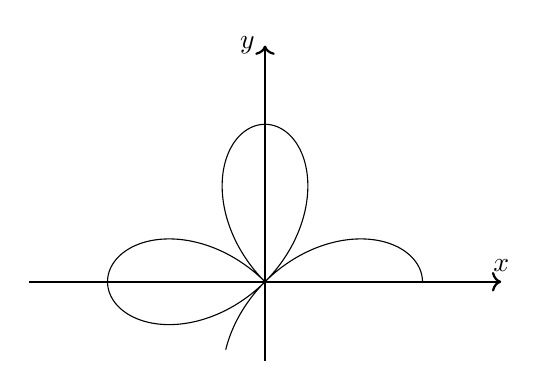
\begin{tikzpicture}
	\draw[thick,->] (-3,0)--(3,0) node[above] {$x$};
	\draw[thick,->] (0,-1)--(0,3) node[left] {$y$};
	\draw[domain=0:4*pi/3,scale=2.0,samples=500] 
		plot ({deg(\x)}:{abs(cos(2*\x r))});
	\end{tikzpicture}
\end{figure}

%		\begin{figure}[htbp]
%		\centering
%		\begin{tikzpicture}
%		\draw[thick,->] (-3,0)--(3,0) node[above] {$x$};
%		\draw[thick,->] (0,-3)--(0,3) node[left] {$y$};
%		\draw[domain=0:2*pi,scale=2.0,samples=500] 
%			plot ({deg(\x)}:{cos(2*\x r)});
%		\end{tikzpicture}
%	\end{figure}

\begin{figure}[htbp]
	\centering
	\begin{tikzpicture}
	\draw[thick,->] (-3,0)--(3,0) node[above] {$x$};
	\draw[thick,->] (0,-1)--(0,3) node[left] {$y$};
	\draw[domain=0:4*pi/3,scale=2.0,samples=500] 
		plot ({deg(\x)}:{abs(sin(2*\x r))});
	\end{tikzpicture}
\end{figure}


		\begin{figure}[htbp]
		\centering
		\begin{tikzpicture}
		\draw[thick,->] (-3,0)--(3,0) node[above] {$x$};
		\draw[thick,->] (0,-1)--(0,3) node[left] {$y$};
		\draw[domain=0:4*pi/3,scale=2.0,samples=500] 
			plot ({deg(\x)}:{acos(sin(\x r))});
		\end{tikzpicture}
	\end{figure}
}


\newpage
\subsection{Arclength - Feb 7}
\begin{definition}
	$f:[a,b]\to \mR$ continuous,
	\[
		\Gamma = \{(x,y): y = f(x), a\leq x \leq b\}
	\]
	$P = \{a = x_0 < \cdots < x_n = b\}$, then 
	\[
		\Length(L_i) = \sqrt{(x_i-x_{i-1})^2 + [f(x_j)-f(x_{j-1})]^2}
	\]
	\[
		\Length(\Gamma) \approx \sum_{j=1}^n length(\L_j) 
		=\sum_{j=1}^n \sqrt{(x_j-x_{j-1})^2 + [f(x_j)-f(x_{j-1})]^2}
	\]
	Add assumptions: 
	\begin{itemize}
		\item f' exists on $[a,b]$ and is continuous on $[a,b]$
	\end{itemize}
	
	\begin{alignat*}{2} 
		M.V.T.
		\Rightarrow &f(x_j-x_{j-1}) = f'(c_j) (x_j-x_{j-1}), \qquad
		c_j\in (x_{j-1}, x_j)\\\\
		%
		\Rightarrow &\sqrt{(x_j-x_{j-1})^2 + [f(x_j)-f(x_{j-1})]^2}\\
			=& \sqrt{(x_j-x_{j-1})^2 + [f'(c_j)(x_j-x_{j-1})]^2}\\
			=& \sqrt{1+f'(c_j)^2}(x_j-x_{j-1})
	\end{alignat*}
	Then, 
	\begin{align*}
		\Length(\Gamma) \approx \sum_{j=1}^n \sqrt{1+[f'(c_j)]^2}
		(x_j-x_{j-1})= S(\sqrt{1+(f')^2}, P)
	\end{align*}
\end{definition}

\begin{definition}
	If $f'$ exists and is continuous on $[a,b]$, $\Gamma = \{(x,y):
	y= f(x), a\leq x \leq b\}$
	\[
		length(\Gamma) = \int_a^b \sqrt{1+[f'(x)]^2}dx
	\]
\end{definition}

{\color{Brown}
	\textbf{Example 1:}
	
	$0\leq \alpha<\beta\leq \pi$, $a > 0$ 
	\[
		\frac{dy}{dx} = \frac{-x}{\sqrt{a^2-x^2}}
	\]
	\begin{align*}
		\Length(\Gamma) 
		=&\int_{a\cos \beta}^{a\cos \alpha} 
		\sqrt{1+(\frac{-x}{\sqrt{a^2-x^2}})^2}dx\\
		%
		=& \int_{a\cos \beta}^{a\cos \alpha} 
		\frac{\alpha}{\sqrt{a^2-x^2}} dx\\
		%
		=& \int_{\beta}^{\alpha} 
		\frac{\alpha}{\sqrt{a^2-a^2\cos^2\theta}}(-a\sin\theta)d\theta\\
		%
		=&\int_{\alpha}^{\beta} \alpha d\theta
		= \alpha(\beta - \alpha)
	\end{align*}
	
	\textbf{Example 2: }
	$\Gamma = \{(x,y):y = x^2, 0\leq x\leq 2\}$, $\frac{dy}{dx} = 2x$
	\[
		\Length(\Gamma)= \int_0^2 \sqrt{1+(2x)^2}dx
	\]
	$2x = \sinh t = \frac{e^t-e^{-t}}2$, $dx = \frac12\cosh t dt$,
	$\cosh t = \frac{e^t+e^{-t}}2$. 
	
	\begin{align*}
		\Length(\Gamma) 
		=& \int_0^{\log(4+\sqrt{17})} \sqrt{1+\sinh^2 t} \frac 12
		\cosh t dt 
		\tag{$t = \log(2x+\sqrt{(2x)^2+1})$}\\
		=& \frac 12 \int_0^{\log(4+\sqrt{17})} \cosh^2 t dt
		\tag{$\cosh^2 t = \frac 12 [\cosh (2t) + 1]$}\\
		=& \frac12 \int_0^{\log(4+\sqrt{17})} [\cosh(2t) + 1]dt
		\tag{$\sinh 2t= 2 \sinh t \cosh t$}\\
		***check***=& \frac 14 \sinh(2t) + 
		t\bigg\vert_0^{\log(4+\sqrt{17})}
	\end{align*}

	\textbf{Method 2}
	$2x = \tan t$, $dx = \frac 12 \sec^2 t dt$, 
	\[
		length(\Gamma) = \int_0^{\arctan(4)} \sqrt{1+\tan^2 t}
		\frac 12 \sec^2 t dt = \frac 12 \int_0^{\arctan (4)}\sec^2 t dt
	\]
	\begin{align*}
		\int \sec^3 t dt 
		=& \int \sec^2 t \sec t dt\\
		=& \tan t \sec t - \int \tan t \tan t\sec t dt\\
		=& \tan \sec t - \int (\sec^3 t - \sec t)dt\\\\
		%
		\Rightarrow 2 \int \sec^3 t dt \\
		=& \tan t \sec t + \int \sec tdt \\
		=& \tan t \sec + \log\abs{\sec t + \tan t} + C\\
		%
		\sec(\arctan 4) =& \sqrt{1+\tan^2(\arctan 4)} = \sqrt{1+16} = \sqrt{17}
	\end{align*}
}

\newpage
\subsection{Parameterization}

We regard $x, y \in [a,b] \to \mR$ (coordinates are each functions)
\[
	\Gamma = \{y(t) : t \in [a,b]\} 
\]
{
\color{Brown}
Examples :

\begin{itemize}
	\item Polar Curves: 
		$x(\theta) = r(\theta)\cos \theta$, 
		$y(\theta) = r(\theta) \sin\theta$. 

	\item Hyperbolic Coordinates: 
		$a, b > 0$, $\frac{x^2}{a^2} - \frac{y^2}{b^2} = 1$

		$x(t) = a\cosh t$\\
		$y(t) = b\sinh t$
\end{itemize}
}

We wish to compute/define $\Length(\Gamma)$,

assumption, 
\begin{itemize}
	\item $x'(t)$, $y'(t)$ always exist on $[a,b]$, $x',y' : [a,b] \to
		\mR$ are each continuous, 
		\[
			P = \{a=t_0<t_1<\cdots<t_n=b\}
		\]
\end{itemize}
\begin{align*}
	length 
	\approx& \sum_{j=1}^n length(L_j)\\
	=& \sum_{j=1}^n \sqrt{[x(t_j) - x(t_{j-1})]^2 + [y(t_j)-y(t_{j-1})]^2}\\\\
	%
	M.V.T. \Rightarrow x(t_j) - x(t_{j-1}) =& x'(c_j) (t_j-t_{j-1}),
	c_j \in (t_{j-1}, t_j)\\
	y(t_j) - y(t_{j-1}) =& y'(c^*_j) (t_j-t_{j-1}),
	c_j^* \in (t_{j-1}, t_j)\\
\end{align*}

\begin{align*}
	length(\Gamma) 
	\approx& \sum_{j=1}^n \sqrt{[x'(c_j)]^2 + [y'(c^*_j)]^2}(t_j-t_{j-1})\\
	\approx& \sum_{j=1}^n \sqrt{[x'(c_j)]^2 + [y'(c_j)]^2}(t_j-t_{j-1})\\
	=& S(\sqrt{(x')^2 + (y')^2}, P) \\\\
	%
	length(\Gamma)
	=& \int_a^b \sqrt{(x'(t)^2 + y'(t)^2} dt
\end{align*}



%------------------------------------------------------------------------------
%------------------------------------------------------------------------------
%------------------------------------------------------------------------------
%------------------------------------------------------------------------------
%------------------------------------------------------------------------------
%------------------------------------------------------------------------------
%------------------------------------------------------------------------------

	\newpage
	\subsection{Volume and Integration}
	\textbf{Volume: }$S \subset \mR^3$ "nice region", typically bounded by
	definable surfaces with definable cross-sections. 

	\[
		Partition = \{a = x_0 < x_1 < \cdots < x_n = b\} = Q 
	\]	
	\[
		\Vol(P) = \sum_{j=1}^n \Vol(P_j) \approx 
		\sum_{j=1}^n A(x_j)(x_j-x_{j-1})
	\]
	
	We define $\Vol(P) = \int_a^b A(x)dx$. 

	\[
		A(x) = \int_{c(x)}^{d(x)}[z_{top, x}(y) - z_{bot, x}(y)]dy
	\]
	Hard Part: Figure out $z_{top, x}, z_{bot, x}, c(x), d(x)$. 

	\textbf{Remark:} we may interchange roles of $x,y,z$. 

	Circular Symmetry: circular symmetry about $x-$ axis, cross sections are 
	circles. 
	
	\textbf{Method of Disks}
	\[
		A(x) = \pi[r(x)]^2
	\]
	\[
		\Vol(S) = \pi\int_a^b [r(x)]^2 dx
	\]

	\textbf{Method of Cylindrical Shells}

	Suppose that $R\subset \mR^3$ is circularly symmetric about $z-axis$. 

	\[
		P = \{0 = x_0 < x_1 < \cdots < x_n = b\}
	\]
	\begin{align*}
		\Vol(R) \approx \sum_{j=1} \Vol(S_j)
		= \sum_{j=1}^n 2\pi t_j h(t_j) (x_j-x_{j-1})\\
		= \sum_{j=1}^n S(H,P) (x_j-x_{j-1})
	\end{align*}
	
	\begin{align*}
		\Vol(S_i) 
		=& \Vol(cylinder, height\  h(t_j), radius \ x_j)
		- \Vol(cylinder, height\ h(t_j), radius \ x_{j-1})\\
		=& \pi x^2_j h(t_j) - \pi x^2_{j-1}h(t_j)\\
		=& \pi(x^2_j-x^2_{j-1})h(t_j)\\
		=& 2\pi \frac{x_j+x_{j+1}}2 (x_j-x_{j-1}) h(t_j)\\
		=& 2\pi t_jh(t_j)(x_j-x_{j-1})
	\end{align*}
	\begin{align*}
		\Vol (R) &= 2\pi \int_0^b xh(x)dx\\
	%
		\Vol (R) &= 2\pi \int_0^b x[z_{top, 0} (x) - z_{bot, 0}(x)]dx
	\end{align*}
%

{\color{Brown}
	\textbf{Example: }
	$S$ a sphere, radius $a > 0$, $x^2+y^2+x^2 = a^2$. 

	Compute volume $(S)$, 

	\textbf{Disks: }
	Fix $x$, for the moment, $-a \leq x \leq a$. Set $y =0$, 
	\[
		x^2+z^2 = a^2 \Rightarrow z^2=a^2-x^2 \Rightarrow r(x) = \sqrt{a^2-x^2}
	\]

	\[
		\Vol(S) = \pi \int_0^a (\sqrt{a^2-x^2})^2dx = \frac 43 \pi a^3
	\]
	
	\textbf{Cylindrical Shells: }
	\begin{align*}
		h(x) =& \sqrt{a^2-x^2}-(-\sqrt{a^2-x^2}) = 2\sqrt{a^2-x^2}\\\\
		%
		\Vol(S) =& 2\pi \int_0^a x 2\sqrt{a^2-x^2}dx \\
		=& 4\pi \int_0^a x\sqrt{a^2-x^2}dx \\
		=& \frac 43 \pi a^3
	\end{align*}

}

\newpage
	\subsection{Application of Antiderivatives: }






%------------------------------------------------------------------------------
%------------------------------------------------------------------------------
%------------------------------------------------------------------------------
%------------------------------------------------------------------------------
%------------------------------------------------------------------------------
%------------------------------------------------------------------------------
%------------------------------------------------------------------------------
%------------------------------------------------------------------------------
%------------------------------------------------------------------------------
%------------------------------------------------------------------------------
%------------------------------------------------------------------------------
%------------------------------------------------------------------------------
\section{DIFFERENTIAL EQUATIONS}
	\subsection{Differential Equations}
	1st order D.E., standard form: 
	\[
		y' = f(x,y) \qquad , \qquad \underbrace{y(x_0) = y_0}_{initial
		value}
	\]
	\textbf{Facts:} 
	\begin{theorem}[\textbf{Caratheodory Existence Theorem:}]
		$f(x,y)$ is continuous near $(x_0, y_0)$ $\Rightarrow$ solution to
		$I.V.P.$ exists. 
	\end{theorem}
	\begin{theorem}[\textbf{Picard-Lindelof Theorem}]
	\end{theorem}
	Nice assumption of $2$nd variable of $f$ near $(x_0, y_0)$. 
	Caratheodory Existence Theroem: 

	{\color{Brown}
	\textbf{Example: }
	$y' = x \cdot y^{\frac 13}$, $y(0)=x_0$

	\textit{Solution \#1:} $y(x) = 0$ 
	
	\textit{Solution \#2:} assume $y(0)\neq 0$, hence $y(x)\neq 0$ in 
	neighborhood of $x$. 
	}



	\newpage
	\subsection{Feb 14}
	An object e.g. person with open parachute falls from a standstill to the 
	earth from height $H$.  (H large $H < R$. ) 

	As the object falls, it experiences wind resistance proportional to
	velocity. 

	


%------------------------------------------------------------------------------
%------------------------------------------------------------------------------
%------------------------------------------------------------------------------
%------------------------------------------------------------------------------
%------------------------------------------------------------------------------
%------------------------------------------------------------------------------
%------------------------------------------------------------------------------

	\newpage
	\subsection{DE - Feb 24}

	\subsubsection{First Order Linear Equation}
	\begin{definition}[\textbf{First Order Linear D.E.}]
		\[
			y' = p(x)y + q(x)  \qquad p, q \ \text{cts functions on some domain}
		\]
		\textbf{Facts:} Any I.V.P. with such a D.E. (i.e. $y(x_0) = y_0$)
		always admits a unique solution, assuming that $p, q$ are continuous in
		the neighborhood of $x_0$.	\\
	\end{definition}
	\begin{algorithm}
	$ $
	\begin{enumerate}
	\item \textbf{Homogeneous Case: }
	$y'=p(x)y$, i.e. $q(x) = 0$, 
	\begin{align*}
		\frac {y'}{y} =& p(x) \\
		\Rightarrow \log\abs{y} =& P(x) + C, P(X) = \int p(x) dx\\
		\Rightarrow y =& ke^{P(x)}, k = e^C > 0
	\end{align*}
	
	\item \textbf{Non Homogeneous Case: }
	Let $P(x) = \int p(x)dx$, as above,
	$y' = p(x) y + \underbrace{q(x)}_{forcing \ term}$ 

	\textbf{"Trick": }
	\begin{align*}
		(d^{-P(x)} y)' 
		=& e^{-P(x)}y' + e^{-P(x)} \cdot (-p(x))\\
		=& e^{-P(x)} (y' - p(x) y) = e^{-P(x)}q(x)\\
		\Rightarrow
		e^{-P(x)} y = &\int e^{-P(x)} q(x)dx \\
		\Rightarrow y =& e^{P(x)} \int e^{-P(x)} q(x)dx
	\end{align*}
	Dont forget the integration constant. 

	$e^{-P(x)} = e^{-\int p(x)dx}$ "integrating factor"	\\
	\end{enumerate}
	\end{algorithm}

	
	{\color{Brown}
	\textbf{Example: }
	Solve $xy' - ey = x^6$, $y' = \frac 3x y + x^5$ 
	\begin{align*}
		p(x) =& \frac 3x \tag{not defined at $x = 0$}\\
		P(x) =& \int \frac 3x dx = 3\log \abs x 
		=\log (\abs x ^3)     \qquad \tag{did not worry about C}\\
	%
		e^{-P(x)} =& \frac1{\abs x^3}\\
		e^{P(x)} =& \abs x^3 \\
		y =& \abs x^3 \int \frac{x^5}{\abs x^3}dx = 
		\begin{cases}
			x^3 [\frac 13 x^3 + C], & x>0\\
			-x^3 [\int \frac{x^5}{-x^3} dx], & x < 0
		\end{cases}
		=
		\begin{cases}
			\frac 13 x^6 + Cx^3, & x>0\\
			\frac 13 x^6 - Cx^3, & x<0
		\end{cases}
	\end{align*}
	Note: equation does not allow $x =0$ in domain, we have for either $x>0$
	or $x<0$. 
	}
	
	\subsubsection{Second Order Linear Equation}

	\begin{definition}[\textbf{Second Order Linear D.E.}]
		\[
			y'' + p(x)y' + q(x) y = r(x) 
		\]
		\textbf{Facts:} 
		\begin{enumerate}
		\item 
		if $p,q,r$ are continuous on an open interval, then a 
		"general solution" exist: $\varphi_1 y_1 + \varphi_2 y_2$, 
		$y_1, y_2$ linearly independent, $\phi_1, \phi_2$ differentible 
		functions, or constants
		\item
			I.V.P $y(x_0) = y_0$, $y'(x_0) = y_0 \Rightarrow$ solution unique.\\
		\end{enumerate}
	\end{definition}
	
	\begin{algorithm}[\textbf{Methods to Solve}]
	$ $
	\begin{enumerate}
		\item \textbf{Homogeneous Case: }
		\[
			y'' + p(x)y' + q(x)y = 0
		\]
		\begin{itemize}
			\item can be very difficult to compute solution unless $p, q,$ are
				constant (A4)
			\item general solution always exists: of form 
				\[
					c_1y_1 + c_2y_2
				\]
				$y_1, y_2$ linearly independent solutions $c_1, c_2$ constants. 
			
				In I.V.P. situation, use initial data to learn $c_1, c_2$.
		\end{itemize}
		
	\item \textbf{Variation of Parameters - L. Euler:}
		
		\[
			y'' + p(x)'y + q(x) y = r(x)  \qquad \heartsuit
		\]

		Idea: replace $c_1, c_2$ from homogeneous case, with functions. 

		We assume: we have $\varphi_1, \varphi_2$ differentiable with continuous
		$\varphi_1', \varphi_2'$, and we consider 
		\[
			y = \varphi_1' y_1 + \varphi_2' y_2 \qquad (f) 
		\]
		$y_1, y_2$ are linearly independent solutions to homogeneous case, and
		\[
			\varphi_1' y_1 + \phi_2'y_2 = 0  \qquad (*)
		\]
		Let's consider for $y$ in (f). 
		\begin{align*}
			y' 
			=& (\varphi_1y_1+\varphi_2y_2) \\
			=& \varphi_1' y_1 + \varphi_2' y_2 + \varphi_1 y_1' +
			\varphi_2 y_2'\\
			=& \varphi_1 y_1' + \varphi_2 y_2' \tag{by (*)} \\
			then \qquad \qquad &\\
			y'' + py' + qy =& \varphi_1'y_1' + \varphi_2'y_2' + \varphi_1y_1''
			+\varphi_2 y_2'' + p(\varphi_1y_1' + \varphi_2 y_2') 
			+ q(\varphi_1y_1 + \varphi_2y_2)\\
			=& \varphi_1'y_1' + \varphi_2'y_2' + \varphi_1(y_1'' + py_1' + qy_1)
			+ \varphi_2(y_2'' + py_2' + qy_2)\\
			=& \varphi_1' y_1' + \varphi_2' y_2' \tag{**}
		\end{align*}
		If we wish to solve $\heartsuit$, then we have 
		\[
			\begin{cases}
				\varphi_1' y_1' + \varphi_2' y_2' = r, \qquad
				by \,\, \heartsuit \,\,  and \,\, **
				\qquad 
				\varphi_1' y_1 + \varphi_2' y_2 = 0 \qquad by \ assumption *
			\end{cases}
		\]
		\[
			\begin{bmatrix}
				y_1 & y_2 \\
				y_1' & y_2'
			\end{bmatrix}
			\begin{bmatrix}
				\varphi_1'\\
				\varphi_2'
			\end{bmatrix}
			=
			\begin{bmatrix}
				0\\
				r
			\end{bmatrix}
			\Rightarrow 
			\begin{matrix}
				\varphi_1' \\
				\varphi_0'
			\end{matrix}
			=\frac1{y_1y_0' - y_1'y_2} 
			\begin{bmatrix}
				y_2' & -y_2\\
				-y_1' & y_1
			\end{bmatrix}
			\begin{bmatrix}
				0\\
				r
			\end{bmatrix}
		\]
		\[
			W = y_1y_2' - y_1'y_2    \qquad Wronskian
			\qquad \Rightarrow 
			\varphi'_1 = -\frac{y_2r}{W}
			\quad \varphi'_2 = \frac{y_1r}{W}
		\]
		
		\begin{align*}
			\varphi_1(x) = -\int\frac{y_2(x)r(x)}{W(x)}dx\\
			\varphi_2(x) = \int\frac{y_1(x)r(x)}{W(x)}dx 
		\end{align*}
		dont forget integraiton constant
		General Solution: 
		\[
			y(x) = \varphi_1(x) y_1(x) + \varphi_2(x)y_2(x)
		\]

		
	\end{enumerate}
	\end{algorithm}





%------------------------------------------------------------------------------
%------------------------------------------------------------------------------
%------------------------------------------------------------------------------
%------------------------------------------------------------------------------
%------------------------------------------------------------------------------
%------------------------------------------------------------------------------
%------------------------------------------------------------------------------
\newpage
\subsection{Feb 26}
\begin{theorem}[\textbf{Taylor's Theorem}]
	Let $I \subseteq \mR$ be an open interval, $f:I\to \mR$, be $(n+1)$-times
	differentiable, then for $a \in \mR$, we have 
	\[
		f(x) 
		= \underbrace{f(a) + f'(a) (x-a) + \frac{f''(x)}2 (x-a)^2 + \cdots + 
		\frac{f^{(n)}(a)}{n!} (x-a)^n}_{P_n(x)} 
		+ \frac{f^{(n+1)}(c)}{(n+1)!} (x-a)^{(n+1)}
	\]
	for all $x \in I$, $c = c_x$ is between $a$ and $x$. 
	\[
		R_n(x) = \frac{f^{(n+1)}(c_x)}{(n+1)!} (x-a)^{n+1}
	\]
	Lagrange Remainder Theorem. 
\end{theorem}
\begin{proof}
	Let $C \in \mR$ satisfy that $f(x) - P_n(x) = C(x-a)^{n+1}$, fix $x$, then
	for $t$ between $a$ and $x$ 
	\[
		\varphi(t) = f(x) - [f(t) + f'(t) (x-t) + \cdots +
		\frac{f^{(n)}(t)}{n!}(x-t)^n + C(x-t)^{n+1}]
	\]
	$\varphi(x) = 0 =\varphi(a)$. Rolle's Theorem $\Rightarrow \varphi'(c) = 0$
	for some $c$ between $a$ and $x$. 

	Calculate: 
	\[
		\varphi'(T) = - \frac{f^{(n+1)}(t)}{n!}(x-t)^n + (n+1)C(x-t)^n
	\]
	Solve to get $C = \dfrac{f^{(n+1)}(c_x)}{(n+1)!}$.\\
\end{proof}

\begin{theorem}[\textbf{Taylor's Theorem version 2}]
	Let $I \subseteq \mR$ be an open interval, $f:I\to \mR$, be $(n+1)$-times
	differentiable with $f^{(n+1)}$ continuous, then for $a \in I$, we have 
	\[
		f(x) = \underbrace{\sum_{k=0}^n \frac{f^{(k)}(a)}{k!} (x-a)^k}_{P_n(x)}
		+ \underbrace{\int_a^x \frac{f^{(n+1)}(t)}{n!} (t-a)^n dt}
		_{R_n(x), \text{Cauchy Form of Remainder for } x\in I }
	\]
\end{theorem}
\begin{proof}
	We have 
	\begin{align*}
		f(x) 
		=& f(a) + \int_a^x f'(t) dt \tag{F.T. of C}\\
		=& f(a) + \int_a^x f'(t)(x-t)^0 dt\\
		=& f(a) - f'(t)(x-t)\bigg\vert_{a=t}^{x=t} + \int_a^x f''(t)(x-t)dt
		\tag{Integration by Parts}\\
		=& f(a) + f'(a)(x-a) + \int_a^x f''(t)(x-t)dt \tag{*}
	\end{align*}
	Inductive Step: 
	\begin{align*}
		\int_a^x f^{(m)}(t) (x-t)^{m-1}dt
		=& -\frac 1m f^{(m)}(t) (x-t)^m \bigg\vert_{t=a}^{t=x}
		+ \frac 1m \int_a^x f^{(m+1)}(t)(x-t)^m dt\\
		=& \frac 1m f^{(m)}(a)(x-a)^m + \frac 1m \int_a^x f^{(m+1)}(t)(t-a)^mdt
	\end{align*}

	\begin{align*}
		* 
		=& f(a) + f'(a)(x-a) + \frac{f''(a)}2 (x-a)^2 + \frac 12 \int_a^x 
		f^{(3)}(t) (x-t)^2 dt\\
		=& f(a) + f'(a)(x-a) + \frac{f''(a)}2(x-a)^2 + \frac 12 [\frac 13 
		f^{(3)}(a)(x-a)^3 + \frac 13 \int_a^x f^{(4)}(a)(x-t)^3 dt] \\
		\vdots &\\
		=& \sum_{k=0}^n \frac{f^{(k)}(a)}{k!} (x-a)^k + \frac 1{n!} \int_a^x
		f^{(n+1)}(t)(x-t)^n dt\\
	\end{align*}
\end{proof}

\textbf{Remark: } we assumed $f^{(n+1)}$ is continuous, the $M/AVT$ for
integrals provides $c = c_x$ between $a$ and $x$ s.t. 
\[
	\frac1{n!} \int_a^x f^{(n+1)}(t)(x-t)^n dt = \frac{f^{(n+1)}(c)}{n!}
	(x-c)^n (x-a) 
\]
above is the second version of Cauchy form of $R_n(x)$.

\textbf{Compare:} lagrange form
\[
	\frac{f^{(n+1)}(c_x)}{(n+1)!} (x-a)^{n+1} = R_n(x) 
	= \frac{f^{(n+1)}(c_x^*)}{n!} (x-c_x^*)^n(x-a) 
\]
$c_x \neq c_x^*$ in general. \\

\begin{proposition}
Given $f:I\to \mR$, $a$ as above, $P_n(x) = \sum_{k=0}^n
\frac{f^{(k)}(a)}{k!} (x-a)^k$, we have that 
\begin{itemize}
	\item $P_n$ is the unique polynomial with $\deg P_n \leq n$ s.t. 
		\[
			\lim_{x\to a} \frac{f(x) - P_n(x)}{(x-a)^n} = 0
		\]
\end{itemize}
\end{proposition}
\begin{proof}
	Suppose $Q$ is polynomial, $\deg Q \leq n$ with 
	\[
		\lim_{x\to a} \frac{f(x)-Q(x)}{(x-a)^n} = 0
	\]
	Then, 
	\[
		Q(x) + [f(x) - Q(x)] = f(x) = P_n(x) + R_n(x) 
		\Rightarrow Q(x) - P_n(x) = R_n(x) - [f(x) - Q(x)]
	\]
	\begin{align*}
		x\neq a \qquad 
		\frac{Q(x) - P_n(x)}{(x-a)^n} 
		=& \frac{R_n(x)}{(x-a)^n} -\frac{f(x)-Q(x)}{(x-a)^n} \\
		=& \frac{\frac{f^{(n+1)}(c_x)}{n!} (x-c_x)^n (x-a)}{(x-a)^n} 
		-\frac{f(x)- Q(x)}{(x-a)^n}\\
		=& \bigg[ \frac{f^{(n+1)}(c_x)}{n!} \cdot \frac{(x-c_x)^n}{(x-a)^n}
		(x-a)\bigg]\\
		=& 0 
	\end{align*}
	and $\deg(Q- P_n)\leq n$, little effort $\Rightarrow Q= P_n$.
\end{proof}

{\color{Brown}
\textbf{Example: }
\[
	e^x = \sum_{k=0}^n \frac1{k!} x^k + \frac{e^c}{(n+1)!} x^{n+1}
\]
$f(x) = e^x$, $f'(x) = e^x$ centered at $a = 0$. 

Wish to examine $e^{-x^2}$. 
\begin{align*}
	e^{-x^2} 
	=& \sum_{k=0}^n \frac1{k!} (-x^2)^k + \frac{e^c}{(n+1)!} (-x^2)^{n+1}\\
	=& \underbrace{\sum_{k=0}^n \frac{(-1)^k}{k!} x^{2k} }_{degree \ 2n}
	+ \frac{e^c\cdot (-1)^{n+1}}{(n+1)!}x^{2n+2} \\
\end{align*}
\textbf{Conclusion:}
\begin{align*}
	\frac{e^{-x^2} - \sum_{k=0}^N \frac{(-1)^k}{k!}x^{2k}}{x^{2n+1}}
	=& \frac{\frac{(-1)^{n+1}e^{c^k}}{(n+1)!}x^{2n+2}}{x^{2n+1}} \\
	\lim_{x \to 0}  \frac{\frac{(-1)^{n+1}e^{c^k}}{(n+1)!}x^{2n+2}}{x^{2n+1}} 
	=& 0\\
\end{align*}
We know that $P_{2n}(x) = \sum_{k=0}^n \frac{(-1)^n}{k!}x^{2k}$, for 
$f(t)=e^{-t^2}$  around $a = 0$. 

We can learn $f^{(k)}(0)$ just from polynomial, for $k = 0, \cdots, n$.
}






%------------------------------------------------------------------------------
%------------------------------------------------------------------------------
%------------------------------------------------------------------------------
%------------------------------------------------------------------------------
%------------------------------------------------------------------------------
%------------------------------------------------------------------------------
%------------------------------------------------------------------------------
\newpage
\subsection{Error Estimation - Feb 28} 

{\color{Brown}
\textbf{Example: } Integral Functions: 
\[
	E(x) = \int_0^x e^{-t^2}dt 
\]
Wish to estimate $E(1)$ with a polynomial in $1$. 

Wish to estimate $E(x)$ with a polynomial in $x$, $x \in [0, 1)$. 

$a = 0$, 
\[
	e^x = \sum_{k=0}^n \frac{x^k}{k!} + \frac{e^c}{(n+1)!} x^{n+1}
\]

\[
	e^{-t^2} = \sum_{k=0}^n \frac{(-1)^k t^{2k}}{k!} + \frac{(-1)^{n+1}e^c}{(n+1)!}
	t^{2n+2}
\]
\begin{align*}
	E(x) 
	=& \int_0^x e^{-t^2}dt = \sum_{k=0}^n \frac{(-1)^k}{k!} \int_0^x t^{2k}dt
	+ \frac{(-1)^{n+1}}{(n+1)!}\int_0^x e^ct^{2n+2} dt	\\\\
	%
	\Rightarrow \qquad \qquad 
	&\abs{E(x) - \sum_{k=0}^n \frac{(-1)^k \cdot x^{2k+1}}{k! \cdot (2k+1)}}\\
	%
	=& \abs{\frac{(-1)^{n+1}}{(n+1)!}\int_0^x e^ct^{2n+2} dt}	\\
	%
	\leq & \frac 1{(n+1)!} \int_0^x \abs{e^ct^{2n+2}} dt\\
	%
	\leq & \frac1{(n+1)!} \int_0^x t^{2n+2} dt, \quad 0 \leq e^c \leq 1,
	\quad c \in [-1, 0]\\
	%
	=& \frac{x^{2n+3}}{(2n+3)(n+1)!} \leq \frac	1{(2n+3)(n+1)!}, 
	\text{as} \ x \in [0, 1]
\end{align*}
\textbf{"Uniform Estimate":} Estimate holds for any $x \in [0, 1]$. 
}

\textbf{Rate of Decay of Estimate:}

Ratio of Estimates: 
\[
	\frac{\frac1{(2(n+1)+3)((n+1)+1)!}}{\frac1{(2n+3)(n+1)!}}
	 = \frac{(2n+3)}{(2n+5)(n+2)} 
\]
Better than exponential decay. 

$e_n$ error in $n$ $e_n \sim r^n$ $(0 < r < 1)$, $\frac{e_{n+1}}{e_n} = r$
(fixed) 



%---------------------------------------S--------------------------------------
%---------------------------------------E--------------------------------------
%---------------------------------------C--------------------------------------
%---------------------------------------T--------------------------------------
%---------------------------------------I--------------------------------------
%---------------------------------------O--------------------------------------
%---------------------------------------N--------------------------------------
%------------------------------------------------------------------------------
%---------------------------------------B--------------------------------------
%---------------------------------------R--------------------------------------
%---------------------------------------E--------------------------------------
%---------------------------------------A--------------------------------------
%---------------------------------------K--------------------------------------
\newpage
\section{SERIES CONVERGENCE}
\subsection{Introduction to Series - Feb 28}
\begin{definition}
	Let $(a_k)_{k=1}^{\infty} \subset \mR$ be a sequence. We define the series
	\[
		\sum_{k=1}^{\infty} a_k := \lim_{n\to\infty} \sum_{k=0}^n a_k
	\]
	provided the limit exists. 

	\textbf{Series = Improper Sum}. 
\end{definition}

\textbf{Terminology:} We say $\sum_{k=1}^{\infty} a_k$ converges provide
$(\sum_{k=1}^n a_k)_{n=1}^{\infty}$ converges.\\

{\color{Brown}
\textbf{Essential Example: Geometric series}

Let $a \in \mR$, when does $\sum_{k=0}^{\infty} a^k$ converges? 

Let $S_n = \sum_{k=0}^n a^k = 1 + a + a^2 + \ldots + a^n$, 

$S_n(1-a) = 1+ + \ldots + a^n - [a+a^2 + \ldots + a^n + a^{n+1}] 
= 1-a^{n+1}$, 
\[
	S_n = 
	\begin{cases}
		\frac{1-a^{n+1}}{1-a}, & if \ a\neq 1\\
		n+1, & if \ a = 1\\
	\end{cases}
\]
\textbf{Fact:} 
\[
	\lim_{n\to\infty} a^{n+1} 
	= 
	\begin{cases}
	0, & \abs{a}<1\\
	D.N.E., & \abs{a} \geq 1, a \neq 1\\
	1, & a = 1
	\end{cases}
\]
Hence, $\sum_{k=0}^{\infty} a^k = \frac1{1-a}$ if $\abs a < 1$. \\

\textbf{Example: } (Sometimes we get lucky)

Consider $\sum_{k=1}^{\infty} \frac1{k(k+1)}$, 
\[
	S_n = \sum_{k=1}^n \frac1{k(k+1)} = \sum_{k=1}^n [\frac 1j - \frac1{k+1}]
	= 1 - \frac 12 + \frac 12 - \ldots + \frac 1n - \frac1{n+1}
\]

\[
	\sum_{k=1}^{\infty} \frac1{k(k+1)} 
	=\lim_{n\to\infty} \sum_{k=1}^n \frac1{k(k+1)} 
	= \lim_{n\to\infty} [1-\frac1{n+1}] = 1
\]
Series converges to 1. 

}




%------------------------------------------------------------------------------
%------------------------------------------------------------------------------
%------------------------------------------------------------------------------
%------------------------------------------------------------------------------
%------------------------------------------------------------------------------
%------------------------------------------------------------------------------
%------------------------------------------------------------------------------
\newpage
\subsection{Series Convergence Test I: NTT and CT - March 2}

\textbf{Recall: }
\[
	\sum_{k=1}^{\infty} a_k := \lim_{n\to\infty} \sum_{k=1}^n a_k
	\quad \text{if limit eixsts. }
\]

\textbf{Fundmanetal Question of Series: Given $\sum_{k=1}^{\infty} a_k$, does 
it converge? }

\textbf{Tests For Convergence: }

\begin{proposition}[\textbf{Test \#1: nth term test - weakest necessity result}]
	\[
		\sum_{k=1}^{\infty} a_j \quad \text{converges}
		\Rightarrow \lim_{k\to\infty} a_k=0
	\]
\end{proposition}
\begin{proof}
	Let $S_n = \sum_{k=1}^N a_k$. Then $a_n = S_n - S_{n-1}$. We assume 
	$\sum_{k=1}^{\infty} a_k= \lim_{n\to\infty} S_n$ exists. 

	Hence $\lim_{n\to\infty} S_{n-1} = \lim_{n\to\infty} S_n$ exists. Hence by
	taking differences of limits of sequences, we get
	\[
		 0 = \lim_{n\to\infty} S_n - \lim_{n\to\infty} S_{n-1}
		 = \lim_{n\to\infty} [S_n - S_{n-1}]
		 = \lim_{n\to\infty} a_n
	\]
\end{proof}

{\color{Brown}
\textbf{Example:} $\abs a \geq 1\Rightarrow \sum_{k=0}^{\infty} a^k$ D.N.E. 
Indeed, $\lim_{k\to\infty} a^k \neq 0$. (or does not exist). }\\

\begin{theorem}[\textbf{Cauchy Criterion for Series Convergence}]
	$\sum_{k=1}^{\infty} a_k \quad \text{converges} \Leftrightarrow$
	given $\ep>0$, there is a $n_{\ep}$ in $\mN$ s.t.
	$\abs{\sum_{k=m}^n a_k} < \ep$. whenever $n > m \geq n_{\ep}$. da
\end{theorem}
\begin{proof}
	let $S_n = \sum_{k=1}^n a_k$. then 
	$\sum_{k=1}^{\infty} a_k$ converges $\Leftrightarrow \lim_{n\to\infty} S_n$
	exists, $\Leftrightarrow$ given $\ep>0$, there is $n_{\ep}$ in $\mN$ so 
	$\abs{S_n - S_{m-1}} < \ep$ whenever $n > ,m \geq n_{\ep}$. 

	Note that $S_n-S_{m-1} = \sum_{k=1}^n a_k - \sum_{k=1}^{n-1} a_k = 
	\sum_{k=m}^n a_k$. \\
\end{proof}

\textbf{Example: }For $\ep = \frac 12 $, then Cauchy Criterion fails for 
$\sum_{k=1}^{\infty} \frac 1k$. \\

\begin{proposition}[\textbf{Linearity of Converging series}]
	Suppose $\sum_{k=1}^{\infty} a_k$ and $\sum_{k=1}^{\infty} b_k$ converges,
	then for $\alpha, \beta \in \mR$, 
	\[
		\sum_{k=1}^{\infty} (\alpha a_1 + \beta b_k) \quad \text{converges}
	\]
	with 
	\[
		\sum_{k=1}^{\infty}(\alpha a_K +\beta b_k)
		= \alpha \sum_{k=1}^{\infty} a_k + \beta \sum_{k=1}^{\infty} b_k
	\]
\end{proposition}
\begin{proof}
	We use linearity of sums and of limits(when they exist). 
	\begin{align*}
		\sum_{k=1}^{\infty} (\alpha a_k + \beta b_k) 
		=& \lim_{n\to\infty} \sum_{k=1}^n (\alpha a_k + \beta b_k)\\
		=& \lim_{n\to\infty} (\alpha \sum_{k=1}^n a_k
		+ \beta \sum_{k=1}^n b_k)\\
		=& \alpha \lim_{n\to\infty} \sum_{k=1}^n a_k
		+ \beta \lim_{n\to\infty} \sum_{k=1}^n b_k \tag{some limit exist}\\
		=& \alpha \sum_{k=1}^{\infty} a_k + \beta \sum_{k=1}^{\infty} b_k\\
	\end{align*}
\end{proof}

\begin{theorem}[\textbf{Comparison Test}]
	Suppose $0\leq a_k \leq b_k$, $k \geq \mN$, for some $N\in \mN$, 
	then 
	\begin{enumerate}
		\item If $\sum_{k=1}^{\infty} b_k$ converges $\Rightarrow 
			\sum_{k=1}^{\infty} a_k$ converges. 
		\item If $\sum_{k=1}^{\infty} a_k$ diverges $\Rightarrow 
			\sum_{k=1}^{\infty} b_k$ diverges.
	\end{enumerate}
\end{theorem}
\begin{proof}
	1. Assume $\sum_{k=1}^{\infty} b_k$ converges, then for $n\geq N$, 
	\begin{align*}
		\sum_{k=1}^n a_k 
		=& \sum_{k=1}^{N-1} a_k + \sum_{k=N}^n a_k		\\
		\leq& \sum_{k=1}^n a_k + \sum_{k=N}^{\infty} b_k	\\
		\leq& \sum_{k=1}^n a_k +\underbrace{\lim_{n\to\infty} \sum_{k=1}^n b_k}
		_{nondecreasing \ in\ n} \\
		\leq& \underbrace{\sum_{k=1}^{N+1} a_k}_{finite}
		+ \underbrace{\sum_{k=1}^{\infty} b_k }_{<\infty}
		\tag{added in $\sum_{k=1}^{\infty} b_k \geq 0$} 
	\end{align*}

	Also $S_{n+1} - S_n = \sum_{k=1}^{n+1} a_k - \sum_{k=1}^n a_k = a_n \geq 0$.
	$\Rightarrow (S_n)_{n=1}^{\infty}$ is non-decreasing. 

	By monotone convergence theorem $\Rightarrow \sum_{k=1}^{\infty} a_n =
	\lim_{n\to\infty} S_n$ exists. 

	2. Assume $\sum_{k=1}^{\infty}a_k$ diverges, since 
	$S_n = \sum_{k=1}^{\infty} a_k$ is non-decreasing, we must have that 
	$\sum_{k=1}^{\infty} a_k = \infty$. Now for $n\geq N$, we have
	\begin{align*}
		\sum_{k=1}^n b_k 
		=& \sum_{k=1}^{N-1}b_k + \sum_{k=N}^n b_k	\\
		\geq& \sum_{k=1}^{N-1} b_k + \sum_{k=N}^n a_k	\\
		=& \underbrace{\sum_{k=1}^{N-1} b_k}_{independent\ of\ n}
		- \underbrace{\sum_{k=1}^{N-1}a_k}_{S_n} + \sum_{k=1}^n a_k 
	\end{align*}
	$\lim_{n\to\infty} \to \infty \Rightarrow \sum_{k=1}^{\infty}b_k = \infty$.
\end{proof}

{\color{Brown}
	\textbf{Example: }
	\[
		\sum_{k=2}^{\infty} \frac 1{(\log k)^k} 
	\]
	\[
		\log k \geq 2 \Leftrightarrow k \geq e^2, i.e. k = \lfloor e^2 \rfloor+1
	\]
	\[
		\frac1{\log k}^k \leq \frac1{2^k}
	\]
	By geometric series of $\frac 12$, the series converges. 

}





%------------------------------------------------------------------------------
%------------------------------------------------------------------------------
%------------------------------------------------------------------------------
%------------------------------------------------------------------------------
%------------------------------------------------------------------------------
%------------------------------------------------------------------------------
%------------------------------------------------------------------------------
\newpage
\subsection{Series Convergence Test II: LCT, RCT, and Ratio Test - March 4}


\textbf{Remark:}
Let $a_k \geq 0$, and $S_n = \sum_{k=1}^n a_k$ 
\[
	S_{n+1} - S_n = a_n \geq 0 \Rightarrow (S_n)_{n=1}^{\infty} is 
	monotone increasing
\]

$\sum_{k=1}^{\infty} S_n$ converges $\Leftrightarrow S_n$ is bounded. 

\begin{corollary}[\textbf{Limit Comparison Test}]
	If $a_k \geq 0$ and $b_k > 0$, and $0 \leq \lim_{k\to \infty} 
	\frac{a_k}{b_k} = L$ exists, then, 
	\begin{enumerate}
		\item If $L > 0$, $\sum_{k=1}^{\infty} b_k$ converges $\Leftrightarrow
			\sum_{k=1}^{\infty} a_k$ converges. 
		\item If $L = 0$, $\sum_{k=1}^{\infty} b_k$ converges $\Rightarrow
			\sum_{k=1}^{\infty} a_k$ converges. 
		\item If $L = 0$, $\sum_{k=1}^{\infty} a_k$ diverges $\Rightarrow
			\sum_{k=1}^{\infty} b_k$ diverges. (Contrapositive of ii). 
	\end{enumerate}
\end{corollary}
\begin{proof}
	1) We suppose $L > 0$, thus there is $N \in \mN$ such that
	\begin{alignat*}{3}
		& & 
		\abs{\frac{a_k}{b_k} - L } <& \frac L2 \qquad \text{if} \quad k \geq N\\
		\Leftrightarrow & \qquad &
		-\frac L2 <& \frac{a_k}{b_k} - L < \frac L2 
		\qquad&  \text{if} &\quad k \geq N\\
		\Leftrightarrow & \qquad & 
		\frac L2 <& \frac{a_k}{b_k} < \frac{3L}2
		\qquad&  \text{if}& \quad k \geq N\\
		\Leftrightarrow & \qquad & 
		\frac{L}2 b_k <& a_k < -\frac{3L}2 b_k 
		\qquad& \text{if} & \quad k \geq N 
	\end{alignat*}
	We have $\sum_{k=1}^{\infty} b_k$  converges
	$\Leftrightarrow \sum_{k=1}^{\infty} \frac L2b_k$ converges, and 
	$\sum_{k=1}^{\infty} \frac{3L}2 b_k$ converges.  
	
	We apply comparison test, twice. \\
\end{proof}

{\color{Brown}
\textbf{Example: }
Let us consider $\sum_{k=1}^{\infty} \frac1{k^p}$, $p \geq 2$, recall that
$\sum_{k=1}^{\infty} \frac1{k(k+1)}$ converges (*). 
\[
	\frac{\frac 1{k^p}}{\frac{1}{k(k+1)}} 
	=\frac{k^2+k}{k^p} 
	=\frac{1+\frac 1k}{k^{p-2}} \overset{k\to\infty}{\rightarrow}
	\begin{cases}
		1,	& p = 2	\\
		0,	& p > 2
	\end{cases}
\]
}
\textbf{Remark: }The limit comparison test is typically easier to compute than
comparison test, and hence useful (you should remember this)\\


\begin{corollary}[\textbf{Ratio Comparison Test}]
	If $a_k > 0$ and $b_k > 0$, and 
	\begin{itemize}
		\item $\frac{a_{k+1}}{a_k} \leq \frac{b_{k+1}}{b_k}$ for 
			$k \geq N$, $N \in \mN$. 
	\end{itemize}
	Then $\sum_{k=1}^{\infty}b_k$ converges $\Rightarrow \sum_{k=1}^{\infty}
	a_k$ converges. 
\end{corollary}
\textbf{Remark:} This is more difficult in practice than either comparison
test or limit comparison test, we will see that it has strong theoretical value.
\begin{proof}
	For $k \geq N$, 
	\begin{alignat*}{2}
		& & \frac{a_{k+1}}{a_k} \leq& \frac{b_{k+1}}{b_k}		\\
		\Rightarrow & \qquad & \frac{a_{k+1}}{b_{k+1}} \leq&\frac{a_k}{b_k}	\\
		\Rightarrow & \qquad & \frac{a_k}{b_k} \leq &\frac{a_N}{b_N} = M
		\qquad for \ k \geq N	\\
		\Rightarrow & \qquad & a_k \geq& Mb_k, \quad for\ k \geq N
	\end{alignat*}
	Then $\sum_{k=1}^{\infty} b_k$ converges 
	$\Rightarrow \sum_{k=1}^{\infty} Mb_k$ converges $\Rightarrow$ 
	comparison test $\sum_{k=1}^{\infty} a_k$ converges.	\\
\end{proof}

\textbf{Main Application of Ratio Comparison Test: }
\begin{theorem}[\textbf{Ratio test}]
	Suppose $a_k > 0$ and that 
	\[
		\lim_{k\to\infty} a_k = r \qquad \text{exists}
	\]
	Then $r \geq 0$, and 
	\begin{enumerate}
		\item If $r < 1 \Rightarrow \sum_{k=1}^{\infty} a_k$ converges,
		\item If $r > 1 \Rightarrow \sum_{k=1}^{\infty} a_k$ diverges.  
	\end{enumerate}
	\textbf{Remark:}
	\begin{itemize}
		\item test is easy to use, as no reference series are required
		\item \textcolor{Orchid}{case $r=1$ is ambiguous
			e.g. $\sum_{k=1}^{\infty} \frac1{k}$ diverges and 
		$\sum_{k=1}^{\infty} \frac1{k(k+1)}$ converges.} 
	\end{itemize}
\end{theorem}

\begin{proof}
	$ $
	\begin{enumerate}
	\item
	Say $r < 1$, pick any $s$ so $r < s < 1$, then there is N in $\mN$, so
	for $k \geq N$, 
	\[
		\frac{a_{k+1}}{a_k} < r-(r-s) = s = \frac{s^{k+1}}{s^k} 
	\]
	We have that $\sum_{k=1}^{\infty} s_k$ converges ($0 < s < 1$), and hence
	by R.L.T. $\sum_{k=1}^{\infty} a_k$ converges too. 

	\item
	Say $r > 1$, pick any $s$ so $1 < s < r$, then there is N in $\mN$, so
	for all $k \geq N$, 
	\[
		\frac{a_{k+1}}{a_k} > r-(r-s) = s = \frac{s^{k+1}}{s^k} 
	\]
	However $\sum_{k=1}^{\infty} s_k$ diverges, If we have that 
	$\sum_{k=1}^{\infty} a_k$ converges, then R.L.T. would imply 
	$\sum_{k=1}^{\infty} S^k$ converges, contradiction.  
	\end{enumerate}
\end{proof}

{\color{Brown}
	\textbf{Example: }
	Consider $\sum_{k=0}^{\infty} \frac{(1000)^k}{\sqrt{k!}}$

	\textbf{Ratio Test: }


}

%------------------------------------------------------------------------------
%------------------------------------------------------------------------------
%------------------------------------------------------------------------------
%------------------------------------------------------------------------------
%------------------------------------------------------------------------------
%------------------------------------------------------------------------------
%------------------------------------------------------------------------------
%------------------------------------------------------------------------------
\subsection{Series Convergence Test III: Integral Test - March 6}

\begin{theorem}[\textbf{Integral Test}]
	Let $a_k > 0$, $k \in \mN$, suppose there is a function $f:[1,\infty) \to
	\mR$ s.t. 
	\begin{itemize}
		\item $f(k) = a_k$ for $k \in \mN$, and
		\item $f$ is non-increasing
	\end{itemize}
	then 
	\[
		\sum_{k=1}^{\infty} a_k \quad \text{converges} \Leftrightarrow
		\int_1^{infty} f(t)dt \quad \text{converges}
	\]
	\textbf{Remark:} $f$ nonincreasing $\Rightarrow$ $f$ is integrable on 
	each $[1,x]$, $x \geq 1$, $A_1$ 
\end{theorem}
\begin{proof}
	$f$ non-increasing, if $t \in [1,\infty]$, find $k \in \mN$, so $t\leq k$,
	then $f(t) \geq f(k) = a_k > 0$, hence, $f(t) > 0$ for $t \in [1,\infty)$.

	If $t\in [k,k+1]$, then 
	\[
		a_k = f(k) \geq f(t) \geq f(k+1) = a_{k+1}
	\]
	and hence, 
	\[
		a_k \geq \int_k^{k+1}f(t)dt \geq a_{k+1} \qquad \text{since}\quad 
		k+1-k=1
	\]
	\begin{align*}
		\sum_{k=1}^{n+1}a_k \geq \int_1^{n+1} f(t)dt 
		= \sum_{k=1}^n \int_k^{k+1}f(t)dt
		\geq \sum_{k=1}^n a_{k+1} = \sum_{k=2}^{n+1}a_k	\tag{*}\\
	\end{align*}
	If $\sum_{k=1}^{\infty} a_k = \lim_{n\to\infty} \sum_{k=1}^{n+1} a_k$
	converges, then, for $x > 1$, 
	\[
		0 \leq \int_1^x f(t)dt \leq \int_0^{\ceil{x}} f(t)dt
		\leq \sum_{k=1}^{\ceil{x}}a_k \overset{x\to\infty}{\longrightarrow}
		\sum_{k=1}^{\infty} a_k < \infty
	\]
	hence $F(x) = \int_1^x f(t)dt$ is increasing, as $F'(x) = f(x) > 0$, and
	$F$ is bounded. 

	Thus $\int_1^{\infty}f(t)dt = \lim_{x\to \infty} F(x)$ converges. 

	Conversely, if $\int_1^{\infty}f(t)dt$ converges, Then for $n \in \mN$,
	\[
		0\leq \sum_{k=1}^{n+1} a_k = a_1 + \sum_{k=2}^{n+1}a_k 
		\leq a_1 + \int_1^{n+1} f(t)dt
		 \overset{x\to\infty}{\longrightarrow}
		 a_1 + \int_1^{\infty} f(t)dt
	\]
	and thus $S_{n+1} = \sum_{k=1}^{n+1}a_k$ is a bounded and non-decreasing 
	sequence, hence, $\sum_{k=1}^{\infty} a_k = \lim_{n\to\infty} S_{n+1}$
	converges. \\
\end{proof}

\textbf{Remark:} Variant: we may mildly weaken assumptions on $f$, above,
If there is $M > 1$, so $f:[M,\infty] \to \mR$ is nondecreasing, 
\begin{itemize}
	\item $f(k) = a_k$, for $k \in \mN$, $k \geq M$, 
\end{itemize}
then $\sum_{k=1}^{\infty} a_k$ converges $\Leftrightarrow$ $\int_1^{\infty} 
f(t)dt$ converges. [exercise]



\begin{corollary}
	If $p > 0$, $\sum_{k=1}^{\infty} \frac1{k^p}$ converges $\Leftrightarrow$
	$p > 1$.
\end{corollary}
\begin{proof}
	$f(t) = \frac1{t^p}$ which is decreasing on $[1,\infty)$.
	
	$f(t) = \frac1{k^p}$, Integral Test: $\sum_{k=1}^{\infty} \frac1{k^p}$
	converges $\Leftrightarrow$ $\int_1^{\infty} \frac{dt}{t^p}$ converges. 

	\[
		\int_1^x \frac{dt}{t^p} = \int_1^x t^{-p}dt
		= 
		\begin{cases}
			\frac 1{1-p} (x^{1-p}-1), & p \neq 1	\\
			\log x, & p = 1
		\end{cases}
		\qquad \overset{x\to\infty}{\longrightarrow} \qquad 
		\begin{cases}
			 \infty, & p\leq 1	\\
			 \frac1{p-1}, & p>1	\\
		\end{cases}
	\]
\end{proof}
{\color{Orchid}
\textbf{Remark:}Indecisive part of ratio test: 
\[
	\frac{\frac{1}{(k+1)^p}}{\frac 1{k^p}}
	=\frac{k^p}{(1+k)^p} = \frac1{(\frac 1k+1)^p}  
	\overset{k\to\infty}{\longrightarrow} 1
\]
}

{\color{Brown}
	\textbf{Example 1:}
	$\sum_{k=1}^{\infty} \frac{k^3+1}{k^5+3k^3+1}$ converges? 
	Use limit comparison test with $\sum_{k=1}^{\infty} \frac1{k^2}$.
	* ratio test fails. 
	
	\textbf{Example 2:}
	Does $\sum_{k=1}^{\infty} ke^{-k^2}$ converge? 
	\begin{enumerate}
		\item integral test
			\[
				\int_1^{\infty} te^{-t^2} = \frac 1{2e} \Rightarrow
				\sum_{k=1}^{\infty} ke^{-k^2} \quad \text{converges}
			\]
		\item ratio test
			\[
				\frac{(k+1)e^{-(k+1)^2}}{ke^{-k^2}} 
				= \frac{k+1}k e^{-2k-1} \overset{k\to\infty}{\longrightarrow}0
				\Rightarrow \quad \text{series converges} 
			\]
		\item limit comparison test
			\[
				\sum_{k=1}^{\infty} e^{-k} \text{converges by geometric series}
			\]
			Know that 
	\end{enumerate}
}
%------------------------------------------------------------------------------
%------------------------------------------------------------------------------
%------------------------------------------------------------------------------
%------------------------------------------------------------------------------
%------------------------------------------------------------------------------
%------------------------------------------------------------------------------
%------------------------------------------------------------------------------
\newpage
\subsection{Series Convergence Test IV: Raabe's Test - March 9}
{\color{Brown}
\textbf{Example:} Euler's Constant

$\gamma = \lim_{n\to\infty} [\sum_{k=1}^n \frac 1k - \log n]$ exists.

\textit{Recall:} \\
$\floor{x} = \max \{k \in \mZ : k \leq x\}$	\\
$\floor(t) \leq t \leq \floor{t} + 1; t \geq 1$\\
$\frac 1{\floor{t}} \geq \frac 1t \geq \frac 1{\floor{t} + 1}$	\\
$\Rightarrow \qquad \frac 1{\floor{t}} - \frac 1t = 0$

Consider 
\begin{align*}
	A_n 
	=& \int_1^n (\frac1{\floor t - \frac 1t} dt)	\\
	=& \int_1^n \frac1{\floor t} dt	\\
	=& \sum_{k=1}^{n-1} \int_k^{k+1} \frac1{\floor t}dt - \log n	\\
	=& \sum{k=1}^{n-1} \frac 1k - \log n	\\\\
\end{align*}
$(A_n = \sum_{k=1}^{n-1} \frac 1k - \log n = 
[\sum_{k=1}^n \frac 1k - \log n] - \frac 1n 
\overset{n\to\infty}{\longrightarrow} \lim_{n\to\infty} 
[\sum_{n=1}^{\infty} \frac 1k - \log n])$

When $a_k > 0$, $\lim_{n\to\infty} \frac{a_{k+1}}{a_k} = 1$. 
(Indeterminate Case of Ratio Test)	\\
}

\begin{proposition}[\textbf{Raabe's Test}]
	Suppose $\lim_{n\to\infty} k (1-\frac{a_{k+1}}{a_k}) = p \in \mR$,
	then 
	\begin{enumerate}
		\item If $p > 1 \Rightarrow \sum_{k=1}^{\infty} a_k$ converges
		\item If $p < 1 \Rightarrow \sum_{k=1}^{\infty} a_k$ diverges
		\item If $p = 1$ and $\abs{k(1-\frac{a_{k+1}}{a_k})-1}\leq \frac mk$ 
			for some $M>0$, then $\sum_{k=1}^{\infty} a_k$ diverges
	\end{enumerate}
	\textit{Remark:} the case $p = \infty$ also gives convergence, the proof is
	similar to $p > 1$ case. 
\end{proposition}
\begin{proof}
	$ $
\begin{enumerate}
\item 
	Let $q>0 \in \mR$, 
	\[
		\frac{\frac 1{(k+1)^q}}{\frac 1{k^q}} = 1-\frac 1k + \frac{B_k}{k^2}
	\]
	where $0 \leq B_k \leq (q+1)1$ (i.e. is bounded).

	Indeed, 
	\[
		\frac{\frac 1{(k+1)^q}}{\frac 1{k^q}} = 
		\frac{(k+1)^q}{k^q}
		= \frac1{(1+\frac1k)^q}
		= (1+\frac 1k)^{-q}
	\]
	Let $f = (1+x)^{-q}$, $f(x) = -q(1+x)^{-q-1}$, $f''(x) = q(q+1)(1+x)^{-q-2}$.

	Taylor's Theorem about $a = 0$: $f(x) = 1-qx \frac{q(q+1)}{(1+cx)^{q+2}}x^2$,
	$cx$ between $0$ and $x$.
	\[
		\frac{\frac 1{(k+1)^q}}{\frac 1{k^q}} 
		= (1+\frac 1k)^{-q}
		= 1- \frac qk + 
		\underbrace{\frac{(q+1)q}{(q+c_k)^{q+2}}}_{B_k, 0\leq B_k \leq q(q+1)}
		\frac 1{k^2} 
	\]

\item
	We write 
	\begin{align*}
		\frac{a_{k+1}}{a_k} 
		=& 1-\frac pk + \frac pk - 1 + \frac{a_{k+1}}{a_k}	\\
	=& 1- \frac pk \frac 1k \underbrace{p-k(1-\frac {a_{k+1}}{a_k}))}_{:=A_k}\\
	=& 1- \frac pk + \frac{A_k}k
	\end{align*}
\[
	\lim_{k\to\infty} A_k = \lim_{k\to\infty} [p-k(1-\frac{a_{k+1}}{a_k})]
	= p - \lim_{k\to\infty} (1-\frac{a_{k+1}}{a_k}) = 0 
	\qquad (By \ Assumption)
\]

\item Let we assume $p > 1$, find $q$ with $p > q > 1$, then 
	$\sum_{k=1}^{\infty} \frac1{k^q}$ converges, and (1, 2) shows that 
	\[
		\frac{\frac 1{(k+1)^q}}{\frac 1{k^q}} - \frac{a_{k+1}}{a_k}
		 = (1-\frac qk + \frac{B_k}{k^2}) - (1-\frac pk + \frac{A_k}k)
		 = \frac{p-q+\frac{B_k}k - A_k}k
	\]
	where $lim_{k\to\infty}(\frac{B_k}k - A_k)=0$.
	
	Hence, $\exists N \in \mN$ s.t. 
	$-\frac{p-q}2 < \frac{B_k}k - A_k < \frac{p-q}2$, so for $k\geq N$.

	\[
		\frac{\frac 1{(k+1)^q}}{\frac 1{k^q}} - \frac{a_{k+1}}{a_k}
		> \frac{p-q}{2k} \Rightarrow 
		\frac{\frac 1{(k+1)^q}}{\frac 1{k^q}} > \frac{a_{k+1}}{a_k}
	\]
	Thus by ratio comparison test, $\frac{a_{k+1}}{a_k}$ converges.

\item 
	If $p<1$, and find $g$ so $p < g < 1$, thus 
	$\sum_{k=1}^{\infty} \frac{1}{k^q}$ diverges. As in II. 
	\[
		\frac{a_{k+1}}{a_k} - \frac{\frac 1{(k+1)^q}}{\frac 1{k^q}} =
		 = \frac{q-p + A_k - \frac{B_k}k}{k}
	\]
	and as $\lim_{k\to\infty} (A_k - \frac{B_k}k) = 0$, $\exists N \in \mN$, 
	so for $k\geq N$, $\frac{q-p}2 < A_k - \frac{B_k}k < \frac{q-p}2$, so
	\[
		\frac{a_{k+1}}{a_k} - \frac{k^q}{(k+1)^q} > 0 \Rightarrow
		\frac{a_{k+1}}{a_k} > \frac{\frac1{(k+1)^q}}{\frac1{k^q}} 
		\Rightarrow \sum_{k=1}^{\infty} a_k 
		\quad \text{diverges}
	\]

\item 
	proof of $3$, We suppose $p = 1$, then 
	\[
		\abs{f(1-\frac{a_{k+1}}{a_k}) - 1} \leq \frac Mk, M >0	
	\]
	\[
		\frac{a_{k+1}}{a_k} = 1-\frac1k + \frac1k(1- k(1-\frac{a_{k+1}}{a_k}))
		\geq 1- \frac 1k - \frac{M}{k^2}
	\]
	Now $\sum_{k = \floor{M} + 2} \frac1{k-M+1}$ diverges. 
\end{enumerate}

\end{proof}

{\color{Brown}
\textbf{Example for Raabe's Test}
Find $a,b \geq 0$, s.t. 
$\sum_{k=1}^{\infty} \frac{(a+1)(a+2)\cdots(a+k)}{(b+1)(b+2)\cdots(b+k)}$ 
converges. 

\[
	\frac{a_{k+1}}{a_k} 
	= \sum_{k=1}^{\infty} 
	\frac{\prod_{i=1}^{k+1} \frac{a+i}{b+i}}{\prod_{i=1}^k \frac{a+i}{b+i}} 
	= \frac{a+k+1}{a+k} \overset{k\to\infty}{\longrightarrow} 1
\]

By Raabe's Test: 
\[
	k(1-\frac{a_{k+1}}{a_k}) = k(1-\frac{a+k+1}{b+k+1})
	= k(\frac{b-a}{b+k+1})
	\overset{k\to\infty}{\longrightarrow}
	b - a
\]
$b-a > 1 \Rightarrow$ converges, and $b-a < 1 \Rightarrow$ diverges.

If $b-a = 1$, 
\[
	k(1-\frac{a_{k+1}}{a_k})-1 = \frac{k(b-a)}{b+k+1} 
	= \frac{(b-a)k - (b+k+1)}{b+k+1}
	= -\frac{b+1}{k+b+1}
\]
\[
	\abs{k(1-\frac{a_{k+1}}{a_k})-1} 
	= \frac{b+1}{k+b+1} = \frac 1k [\frac{b+1}{1+\frac{b+1}k}]
	< \frac{b+1}k
\]
$b-a=1 \Rightarrow$ converges.
}	\\



%------------------------------------------------------------------------------
%------------------------------------------------------------------------------
%------------------------------------------------------------------------------
%------------------------------------------------------------------------------
%------------------------------------------------------------------------------
%------------------------------------------------------------------------------
%------------------------------------------------------------------------------
\newpage
\subsection{Serires Convergence Test V: AST - March 11}

\begin{theorem}[\textbf{Leibnitz Alternating Series Test}]
	Suppose 
	\begin{itemize}
		\item $a_1 \geq a_2 \geq \cdots \geq 0$
		\item $\lim_{k\to\infty} a_k = 0$
	\end{itemize}
	then, $\sum_{k=1}^{\infty} (-1)^{k+1} a_k$ converges.
	
	Furthermore, $\abs{\sum_{k=1}^{\infty} (-1)^{k+1} a_k}\leq a_1$. 
\end{theorem}
\begin{proof}
	We let $S_n = \sum_{k=1}^n (-1)^{k+1}a_k$, then 
	\begin{align*}
		S_{2n} \leq& S_{2n} + a_{2n+1} - a_{2n+2}	\\
		=& S_{2n+2}	\\
		=& a_1 - a_2 + a_3 - a_4 + \cdots - a_{2n} + a_{2n+1} - a_{2n+2}	\\
		=& a_1 - (a_2-a_3) - (a_4-a_5) -\cdots -(a_{2n} -a_{2n+1})-a_{2n+2}	\\
		\leq & a_1
	\end{align*}

	Hence, $0 \leq S_2 \leq S_{2n+2} \leq a_1$, i.e. $(S_{2n})_{n=1}^{\infty}$
	is non-negative, non-decreasing, and bounded. 

	Monotone Convergence $\Rightarrow \alpha = \lim_{n\to\infty} S_{2n}
	\leq a_1$ exists. 
	\[
		\abs {\alpha - S_{2k}} < \frac{\ep}2, \quad a_{2k+1}< \frac{\ep}2,
		\qquad \text{whenver} \ k \geq N. 
	\]
	If $n\geq 2N+1$, and with $k = \floor{\frac n2} \geq N$, we have

	\[
		S_n 
		= 
		\begin{cases}
			S_{2k}, &n  \text{ even}		\\
			S_{2k=1}, &n \text{ odd}
		\end{cases}
	\]
	and thus 
	\[
		\abs{L-S_n} = \begin{cases}
		\abs{L-S_{2k}}, & n \text{even}	\\
		\abs{L-S_{2k} - a_{2k+1}}, & n \text{odd}
		\end{cases}
		< 
		\begin{cases}
			\frac{\ep}2	\\
			\frac{\ep}2 + \frac{\ep}2 
		\end{cases}
		\leq \ep
	\]
	So we conclude that $\lim_{n\to\infty} (-1)^{k+1}a_{k} = L$. 
\end{proof}

\begin{corollary}
	Let $(a_n)_{n=1}^{\infty} \subset \mR$ satisfy that 
	\begin{itemize}
		\item $a_k$ is eventually non-increasing, non-negative, there is $N \in
			\mN$, $a_k \geq a_{k+1} \geq 0$ if $k \geq N$. 
		\item $\lim_{k\to\infty} a_n = 0$,
	\end{itemize}
	then, 
	\begin{enumerate}
		\item $\sum_{k=1}^{\infty} (-1)^{k+1}a_k$ converges
		\item Error estimate: if $m \geq N$, $\abs{\sum_{k=m}^{\infty}(-1)^k a_k}
			\leq a_m$
	\end{enumerate}
\end{corollary}
\begin{proof}
	Let $n > m \geq N$, 
	\begin{align*}
		\sum_{k=1}^n (-1)^{k+1}a_k 
		=& \sum_{k=1}^n (-1)^{k+1}a_k + \sum_{k=m+1}^n(-1)^{k+1} a_k	\\
		=& \sum_{k=1}^n (-1)^{k+1}a_k + (-1)^m \sum_{k=m+1}^n(-1)^{k-m+1} a_k\\\\
		%
		\lim_{n\to\infty} \sum_{k=m+1}^n(-1)^{k-m+1} a_k 
		=& \lim_{n\to\infty} \sum_{l=1}^{n-m} (-1)^{l+1} a_{l+m}	\\
		=& \sum_{l=1}^{\infty} (-1)^{l+1} a_{l+m} \in [0, a_{m+1}]
	\end{align*}
\end{proof}

{\color{Brown}
\textbf{Example: }
Let $F(x) = \int_0^x \sin(\frac 1t) dt$.

FTofCI, $x \neq 0$, $F'(x) = \sin(\frac 1t)$, as $x\mapsto \sin(\frac 1x)$ is 
continuous away from $0$. 

Notice that the integrand is not continuous at $x = 0$, can we evaluate
$F'(0)$?  

\textit{Answer:} $F'(0) = 0$. 

Notice that 
\[
	F(-x) = \int_0^{-x} \sin (\frac 1t)dt = \int_0^x \sin(-\frac 1u)du
	= \int_0^x \sin(\frac 1u)du = F(x)
\]
so $F$ is even, also, $F(0) = 0$, want 
\[
	\lim_{x\to 0} \frac{F(x) - F(0)}{x-0} 
	= \lim_{x\to 0} \frac{F(x)}x 
\]
We will assess $\lim_{x\to 0^+} \frac{F(x)}x$. 

Set $x > 0$, since $t \mapsto \sin(\frac 1t)$ is bounded and continuous on
$(o,x]$,
\[
	F(x) = \int_0^x \sin(\frac 1t)dt
	= \lim_{u\to 0^+} \int_u^x \sin(\frac 1t)dt
\]
Since 
\[
	F(x) = \lim_{n\to\infty} \int_{\frac1{(n+1)\pi}}^x \sin (\frac 1t)dt 
	= \lim_{n\to\infty}
	\left[
		\sum_{k=k_x}^n \int_{\frac1{(k+1)\pi}}^{\frac 1{k\pi}} 
		\sin(\frac 1t)dt 
		+ 
		\int_{\frac1{k_x\pi}}^x \sin (\frac 1t)dt
	\right]
\]
where $k_x$ in $\mN$ satisfy that 
\begin{align*}
	& &\frac1{k_x\pi} \leq x <& \frac 1{(k_x-1)\pi}	\\
	\Rightarrow &	&\frac 1{k\pi} \leq& k_x	\\
	\Rightarrow &	&k_x - 1 <& \frac 1{k\pi}	\\
	\Rightarrow &	&k_x =& \ceil{\frac1{k\pi}}	\geq \frac1{x\pi}
\end{align*}
let 
\[
	a_k = \int_{\frac1{(k+1)\pi}}^{\frac 1{k\pi}} \abs{\sin(\frac 1t)}dt > 0
\]
\[
	\sum_{k=k_x} \int_{\frac1{(k+1)\pi}}^{\frac 1{k\pi}} \sin(\frac 1t)dt 
	=\sum_{k=k_x}^n (-1)^k a_k
\]
Now 
\begin{align*}
	a_{k+1} 
	=& \int_{\frac1{(k+2)\pi}}^{\frac 1{(k+1)\pi}} \abs{\sin(\frac 1t)dt}	\\
	=& \frac k{k+2} 
	\int_{\frac1{(k+1)\pi}}^{\frac 1{k\pi}} \abs{\sin(\frac 1u)}du< a_k		\\\\
	%
	u =& \frac{\frac1{k\pi}-\frac1{(k+1)\pi}}{\frac1{(k+1)\pi}-\frac1{(k+2)\pi}}
	- (t - \frac 1{(k+2)\pi}) + \frac 1{(k+1)\pi}	\\
	=& \frac{k+2}k (t- \frac1{(k+2)\pi}) + \frac1{(k+1)\pi} 
	\Rightarrow \frac{k+2}k dt
\end{align*}
Hence,r
}


%------------------------------------------------------------------------------
%------------------------------------------------------------------------------
%------------------------------------------------------------------------------
%------------------------------------------------------------------------------
%------------------------------------------------------------------------------
%------------------------------------------------------------------------------
%------------------------------------------------------------------------------
%------------------------------------------------------------------------------
\newpage
\subsection{March 12}
\begin{proposition}[\textbf{Arbitrary Rearrangement}]
	If $\sum_{k=1}^{\infty} a_k$ converges absolutely, and let $\sigma :\mN
	\to \mN$ be one-to-one and onto, (arbitrary rearrangement of $\mN$), then
	$\sum_{k=1}^{\infty} a_{\sigma}(k)$ converges, to the value of 
	$\sum_{k=1}^{\infty} a_k$. 
\end{proposition}
\begin{proof}
	We start with Cauchy Criterion, given $\ep > 0$, there is $N$ in $\mN$, 
	s.t. 
	\[
		\sum_{k=m}^n \abs{a_k} < \frac{\ep}2 \qquad 
		\text{whenever } n > m \geq N
	\]
	We next choose $N_{\sigma}$ s.t. 
	\[
		\{1, \ldots, N\} \subseteq 
		\{\sigma(1), \sigma (2), \ldots, \sigma(N_{\sigma})\}
	\]
	[ontoness of $\sigma$ is required]. Thus we let $n > N_{\sigma} \geq N$,
	then. 
	\begin{align*}
		\abs{\sum_{k=1}^n a_k - \sum_{k=1}^n a_{\sigma(k)}}
		=& \abs{\sum_{k=N+1}^n a_k - \sum_{k=1}^n a_{\sigma(k)}}	\\
		\leq& \sum_{k=N+1} \abs{a_k} +
		\sum_{k = N+1}^{\max\{\sigma(j) : j=1,\ldots, N\}} \abs{a_k}	\\
		<& \frac{\ep}2 + \frac{\ep}2 = \ep
	\end{align*}
	it follows that 
	$\sum_{k=1}^{\infty} a_k = \lim_{a\to\infty} \sum_{k=1}^n a_k 
	= \lim_{k\to\infty} \sum_{k=1}^n a_{\sigma(k)} = \sum_{k=1}^{\infty}
	= \sum_{k=1}^{\infty} a_{\sigma(k)}$. 

\end{proof}


\textbf{\textit{Remark:}} 

We say that $\sum_{k=1}^{\infty} a_k$ is 
\textbf{conditionally convergent} if it is convergent, but not absolutely
convergent. 

{\color{Brown}
	\textbf{Example:}
	$\sum_{k=1}^n \frac{(-1)^k}k$ (L.A.S.T $\Rightarrow$ convergent), if fact,
	$= -\log 2$(A4)
}

if $\sum_{k=1}^{\infty}a_k$ is conditionally convergent, and $\alpha\in\mR$(any
$\alpha$ will do). then there exists a rearrangement $\sigma_{\alpha}:\mN\to
\mN$ s.t. 
\[
	\sum_{k=1}^{\infty} = a_{\sigma(k)} = \alpha
\]

\begin{proposition}[\textbf{Cauchy Product Formula}]
Let $\sum_{k=0}^{\infty} a_k, \sum_{l=0}^{\infty}b_k$ each be absolutely 
convergent, then,
\[
	\sum_{k=0}^{\infty} a_k \ldots \sum_{l=0}^{\infty}b_k
	= \sum_{k=0}^{\infty} (\sum_{j=0}^{k} a_jb_{k-j})
\]
\end{proposition}
\begin{proof}
	Let $N \in \mN$ be so for $n>m \geq N$ we have 
	\[
		\sum_{k=m}^n \abs{a_k} < \sqrt{\ep}, \sum_{l=m}^n \abs{b_l}<\sqrt{\ep}
	\]
	$n \in \mN$, 
	\[
		\sum_{k=0}^{n} a_k \cdot \sum_{l=0}^n b_l
		= \sum_{k=0}^n \sum_{l=0}^n a_kb_l
	\]
	Now let $n\geq 2N+2$, $\frac n2 \geq N+1\Rightarrow \floor{\frac n2}\geq N$.
	\begin{align*}
		& \abs{\sum_{k=0}^n a_k \cdot \sum_{l=0}^n b_k - \sum_{k=0}^{n}
		(\sum_{j=0}^k a_jb_{k-j})}	\\
		=& \abs{\sum_{k,l=1, k+l>n}^n a_kb_l}
		\leq \sum_{k,l=1, k+l>n}^n \abs{a_k}\abs{b_l}	\\
		\leq& \sum_{k=\floor{\frac n2}}^n \abs{a_k} \cdot 
		\sum_{l = \floor{\frac n2}} < \sqrt{\ep} \cdot \sqrt{\ep} = \ep
	\end{align*}
	\begin{align*}
		\sum_{k=0}^{\infty} a_k \cdot \sum_{l=0}^{\infty} b_l
		=& \lim_{n\to\infty} \sum_{k=0}^{\infty} a_k\cdot \sum_{l=0}^n b_l \\
		=& \lim_{n\to\infty} \sum_{k=0}^{\infty} (\sum_{j=0}^k a_j b_{k-j})	\\
		=& \sum_{k=0}^{\infty}(\sum_{j=0}^k a_j b_{k-j})
	\end{align*}
\end{proof}


\begin{definition}
	Let $f:[1,\infty) \to\mR$, be integrable on $[1,x]$, $x > 1$, we say that
	$\int_1^{\infty} f$ converges absolutely, if $\int_1^{\infty}\abs{f}$
	converges. \\
\end{definition}

\begin{proposition}
	With $f$ satisfying first assumption above, t$\int_1^{\infty}$ converges
	absolutely $\Rightarrow \int_1^{\infty} f$ converges. 
\end{proposition}
\begin{proof}\textbf{Cauchy Criterion}

	Given $\ep > 0$, there is $M > 1$ s.t. 
	\[
		\int_u^v \abs f < \ep \qquad 
		\text{whenever} v > u \geq M
	\]
	hence, 
	\[
		\abs{\int_u^v f} \leq \int_u^v \abs{f} < \ep
		\qquad 
		\text{if}
		\quad 
		v > u \geq M
	\]
	Thus $F()x = \int_1^x f$ converges as $x \to \infty$.
\end{proof}

\begin{proposition}
	Let $f$ satisfy first assumption ab ove, if there is $g:[1,\infty) \to
	\mR$, then 
	\begin{itemize}
		\item $\abs{f(t)} \leq g(t)$
		\item $\int_1^{\infty} g$ converges
	\end{itemize}
\end{proposition}




\section{SERIES AND FUNCTION}
\subsection{Pointwise Convergence and Integral Test Revisited - March 23}
{\color{Brown}
	\textbf{Example: } Does $\sum_{k=2}^{\infty} \frac1{(\log k)^{\log k}}$
	converge? 
}

{\color{Orchid}
\textit{Remark: } The integral Test is useful and works in both directions.\\ 
}

\begin{definition}[\textbf{Pointwise Convergence}]
	Let $f_1, f_2, \ldots$  and $f$ be functions on an interval $I$. We say
	that
	\[
		\lim_{n\to\infty} f_n = f \text{ \textbf{pointwise} on } I,
		\text{ if } \lim_{n\to\infty} f_n(x) = f(x)
		\text{ for each } x \text{ in } I
	\]\\
\end{definition}


{\color{Orchid}
\textit{Remark:}
1. Pointwise Convergence is highly unstable. \\
2. The pointwise limit of differentiable/continuous functions need not be 
continuous. 
}




%------------------------------------------------------------------------------
%------------------------------------------------------------------------------
%------------------------------------------------------------------------------
%------------------------------------------------------------------------------
%------------------------------------------------------------------------------
%------------------------------------------------------------------------------
%------------------------------------------------------------------------------d\newpage
\subsection{Uniform Convergence}
\begin{definition}[\textbf{Uniform Convergence}]
	Let $f_1, f_2, \ldots$, and $f$ be functions on a interval $I$. We say that
	\[
		\lim_{n\to\infty} f_n = f \text{ uniformly on I} 
	\]
	if given $\ep > 0$, there is $N$ in $\mN$ for which 
	\[
		\abs{f_n(x) - f(x) < \ep)} \text{ for every } x \text{ in } I, 
		\text{whenever } n \geq N
	\]
	i.e.
	\[
		f(x) - \ep < f_n(x) < f(x) + \ep \text{ for every } x \text{ in }
		I, \text{ whenever } n \geq N
	\]
	Hence, for $n\geq N$, we have
	\[
		\{(x , f_n(x)) : x \in I\} 
		\subset 
		\{(x, y) : f(x) - \ep < y < f(x) + \ep : x \in I)\}
		\\
	\]
\end{definition}

\begin{theorem}[\textbf{Uniform Convergence and Integrals}]
	Let $f_1, f_2, \ldots$ and $f$ be functions on $[a, b]$, such that
	\begin{itemize}
		\item each of $f, f_1, f_2, \ldots$ are integrable on $[a,b]$ and
		\item $\lim_{n\to\infty} = f$ uniformly on $[a,b]$.
	\end{itemize}
	then, 
	\[
		\lim_{n\to\infty} \int_a^b f_n = \int_a^b f \,\, .
	\]
\end{theorem}
\begin{proof}
	We use uniform convergence: given $\ep > 0$ there is $N$ be so that
	\[
		\abs{f_n (x) - f(x)} < \frac{\ep}{b-a+1} \text{ for every } x 
		\text{ in } [a, b], \text{ whenever } n \geq N
	\]
	Thus, if $n \geq N$, we use linearity and order properties of integrals to 
	see that 
	\[
		\abs{\int_a^b f_n - \int_a^b f} = \abs{\int_a^b (f_n - f)}
		\leq \int_a^b \abs{f_n - f} \leq \int_a^b \frac{\ep}{b-a+1} < \ep
	\]
	hence, $\lim_{n\to\infty} \int_a^b f_n = \int_a^b f$.
\end{proof}

\begin{theorem}[\textbf{Uniform Convergence and Continuity}]
	Let $f_1, f_2, \ldots, $ and $f$ be functions on an interval $I$, such that
	\begin{itemize}
		\item each of $f_1, f_2, \ldots$ is continuous on $I$, and 
		\item $\lim_{n\to\infty} f_n = f$ uniformly on $I$.
	\end{itemize}
	Then, $f$ is continuous on $I$. 
\end{theorem}
\begin{proof}
	Fix $x_0$ in $I$ and $\ep > 0$, then uniform convergence provides $N$ in 
	$\mathbb{N}$ for which 
	\[
		\abs{f_n(x) - f(x)} < \frac{\ep}3 \text{ for every } x \text{ in }
		I, \text{ whenever } n \geq N. 
	\]
	Next, we let $\delta > 0$ satisfy the definition of continuity of $f_N$ at
	$x_0$: 
	\[
		\abs{f_N(x) - f_N(x_0)} < \frac{\ep}3 \text{ whenever } x \in I, 
		\abs{x - x_0} < \delta \,\, .
	\]
	Let $ x\in I$, $\abs{x - x_0} < \delta$, then, 
	\begin{align*}
		&\abs{f(x) - f(x_0)}
		\\
		\leq& \abs{f(x) - f_N(x)} + \abs{f_N(x) -f(x_0)}
		\\
		<& \frac{\ep}3 + \frac{\ep}3 + \frac{\ep}3 = \ep \,\, , 
	\end{align*}
	this shows that $f$ is continuous at $x_0$. THis is true for any $x_0$ in 
	$[a,b]$, we see that $f$ is continuous on $[a,b]$.	\\
\end{proof}

\begin{theorem}[\textbf{Weierstrass M-Test}]
	Let $f_1, f_2, \ldots $ be functions on an interval $I$, such that 
	there are $M_1, M_2, \ldots$, such that each $\sup_{x \in I} \abs{f_k(x)}
	\leq M_k$ and $M = \sum_{k = 1}^{\infty} M_k$ converges. 
	then there is a function $f: I \to \mR$ such that 
	\[
		\sum_{k=1}^{\infty} f_k = \lim_{n\to\infty} \sum_{k=1}^{n} f_k = f
		\text{ uniformly on } I \,\, ,
	\]
	In particular, if each $f_k$ is continuous, then so too is $f$. 
\end{theorem}
\begin{proof}
	For each $x$ in $I$, $\abs{f_k(x)} \leq M_k$ so $\sum_{k=1}^{\infty} f_k(x)$,
	by Comparison test. Define $f(x) = \sum_{k=1}^{\infty} f_k(x)$ for $x$ in
	$I$. 

	Given $\ep > 0$, there is $N$ in $\mN$ such that for $m\geq N$ we have
	\[
		\ep > \abs{M - \sum_{k=1}^m M_k} = \abs{\sum_{k=m+1}^{\infty} M_k}
		= \sum_{k = m+1} ^{\infty} M_k
	\]
	Hence $n \geq N$ we have for any $x \in I$ that 
	\begin{align*}
		\abs{f(x) - \sum_{k=1}^{m} f_k(x)} 
		=& \abs{\sum_{k=1}^m f_k(x)}\\
		=& \abs{\lim_{n\to\infty} \sum_{k=m+1}^n f_k(x)}\\
		\leq & \lim_{n\to\infty} \sum_{k=m+1}^n \abs{f_k(x)}
		\leq \lim_{n\to\infty} \sum_{k=m+1}^n M_k	\\
		=& \sum_{k=m+1}^{\infty} M_j < \ep
	\end{align*}
	Notice that the above estimate is for every $x$ in $I$, and hence, we get
	$f = \lim_{m\to\infty} \sum_{k=1} f_k = \sum_{k=1}^{\infty} f_k$ uniformly
	on $I$. 

	In each $f_k$ is continuous, then each $\sum_{k=1}^m f_k$ is continuous, 
	and the Theorem on \textit{Uniform Convergence and Continuity} shows that
	$f$ must be, too. 
\end{proof}

\textbf{Summary: }







%------------------------------------------------------------------------------
%------------------------------------------------------------------------------
%------------------------------------------------------------------------------
%------------------------------------------------------------------------------
%------------------------------------------------------------------------------
%------------------------------------------------------------------------------
%------------------------------------------------------------------------------
\newpage
\subsection{Power Series and Taylor Series - March 27}

\begin{definition}
	A power series about $a$ in $\mR$ is any function defined in a
	neighborhood of $a$ of the form
	\[
		f(x) = \sum_{k=0}^{\infty} a_k(x-a)^k 
	\]
	where $(a_k)_{k=0}^{\infty} \subset \mR$. This being a series, the 
	determination of when it converges is an issue. 

	\textbf{Radius of Convergence: } 
	\[
		R = \frac 1{\limsup _{k\to\infty} \sqrt[k]{\abs{a_k}}}
		= \lim_{k\to\infty} \frac{\abs{a_k}}{\abs{a_{k+1}}}
		\text{ if the limit exists} \,\, .
	\]
	Give a power series $f(x)$ as in ($\heartsuit$) with radius of convergence
	$R$, we have that 
	\[
		f(x) = \sum_{k\to\infty}^{\infty} a_k(x-1)^k 
		\begin{cases}
			\text{converges if } \abs{x-a} < R	\\
			\text{diverges if } \abs{x-a} > R
		\end{cases}
	\]\\ 
\end{definition}


\begin{theorem}[\textbf{Convergence of Power Series}]
	Let $f(x) = \sum_{k=0}^{\infty} a_k(x-a)^k$ be a power series with radius
	of convergence $R > 0$. Then for any $0 < r < R$ we have that 
	\[
		f(x) = \lim_{n\to\infty} a_k (x-a)^k 
		\text{ uniformly on } [a-r, a+r]
	\]
	In particular, $f$ is continuous on $(a-R, a+R)$. 
\end{theorem}
\begin{proof}
	The heart of this proof is the Weierstrass M-Test. 

	Since $r < R$ we exploit the method by which we devised $R$.
	
\end{proof}




\begin{definition}[\textbf{Taylor Series}] 
	The \textbf{Taylor Series} of $f$ about $a$ by 
	\[
		\sum_{k=0}^{\infty} \frac{f^{(k)}(a)}{k!} (x-a)^k \,\, .
	\]
\end{definition}



\begin{proposition}
	Suppose $f$ as above admits $r>0$ for which the remainder terms admits 
	uniform bound
	\[
		\abs{R_n(x)} = \abs{\frac{f^{(n+1)}(c_x)}{(n+1)!} (x-a)^{n+1}} 
		\leq M_n 
		\text{ for } \abs{x-a} \leq r 
		\text{ where } \lim_{n\to\infty} M_n = 0
	\]
	then the radius of convergence of the Taylor series satisfies $R > r$, and
	\[
		f(x) = \sum_{k=0}^{\infty} \frac{f^{(k)}(a)}{k!} (x-a)^k 
		\text{ for } \abs{x-a} \leq r
	\]
\end{proposition}


\begin{lemma}
	Let $(a_k)^{\infty}_{k=0} \subset \mR$, then the power series
	\[
	f(x) = \sum_{k=1}^{\infty} k a_k (x-a)^{k-1} 
	\text{ converges } 
	\Leftrightarrow (x-a)g(x) = \sum_{k=1}^{\infty} ka_k(x-a)^k 
	\text{ converges} 
	\]
	admit the same radius. 
\end{lemma}



\begin{theorem}[\textbf{Derivative and Interals of Power Series}]
	Let $f(x) = \sum_{k=0}^{\infty} a_k (x-a)^k$ have radisu of convergence 
	$R > 0$. Then, 
	\begin{enumerate}
		\item for $x \in (a-R, a+R)$, $\int_a^x f(t) dt = \sum_{k=0}^{\infty}
			\frac{a_k}{k+1} (x-a)^{k+1}$, 
		\item $f$ is differentiable on $(a-R, a+R)$ with $f'(x) = \sum_{k=1}
			^{\infty} ka_k (x-a)^{k-1}$. 
	\end{enumerate}
\end{theorem}
\begin{proof}
	\begin{enumerate}
		\item Since $f_n(x) = \sum_{k=0}^n a_k(x-a)^k$, above, converge 
			uniformly on $[a,x]$ for each $x$ in $(a-R, a+R)$, we can use 
			Uniform Convergence and Integrals to see that
			\begin{align*}
				\int_a^x f(t) dt 
				=& \int_a^x \lim_{n\to\infty} \sum_{k=0}^n a_k (k-a)^k dt 
				\\
				=& \lim_{n\to\infty} \int_a^x \sum_{k=0}^n \frac{a_k}{k+1}
				(x-a)^{k+1}
				\\
				=& \sum_{k=0}^{\infty} \frac{a_k}{k+1} (x-a)^{k+1} 
			\end{align*}

		\item The function $f_n$ above satisfy $f_n'(x) = \sum_{k=1}^n ka_k
			(x-a)^{k-1}$. Let 
			\[
				g(x) = \sum_{k=1}^{\infty} k a_k (x-a)^{k-1}
			\]
			as in the Lemma above, then by Convergence of Power Series we have
			that 
			\[
				\lim_{n\to\infty} f'_n = f 
				\text{ uniformly on } [a-r, a+r] 
				\text{ for } 0 < r < R
			\]
			Since each $f_n(a) = a_0$, we apply F.T. of C. II to each
			$f_n'$, and then Uniform Convergence and Integrals to see for $x$
			in $(a-R, a+R)$ that 
			\[
				f(x) = \lim_{n\to\infty} f_n(x) = \lim_{n\to\infty} 
				= \lim_{n\to\infty} [a_0 + \int_a^x f'_n(t)dt]
				= a_0 + \int_a^ x g(t) dt
			\]
			but then, by F.T.of C.I, we see that
			\[
				f'(x) = g(x) = \sum_{k=1}^{\infty} ka_k (x-a)^{k-1} .
			\]	
	\end{enumerate}
\end{proof}


\begin{corollary}
	Let $f(x) = \sum_{k=0}^{\infty} a_k (x-a)^k$ be as above, then 
	\[
		a_k = \frac{f^{(k)}(a)}{k!} 
		\text{ for each } k = 0, 1, 2, \ldots 
	\]
	In particular, the power series representation for $f$ is unique on 
	$(a - R, a + R)$. 
\end{corollary}
\begin{proof}
	A simple induction shows that 
	\[
		f(a) = a_0, \qquad f'(a) = a_1, \qquad f''(a) = 2a_2. 
		\qquad 
		\ldots, 
		\qquad 
		f^{(k)}(a) = k!a_k
	\]
\end{proof}


\begin{proposition}
	Suppose $f$ is in infinitely differentiable in a neighbourhood of $a$ and
	admits $r > 0$ for which the remainder terms admit uniform bounds:
	\[
		\abs{R_n(x)} 
		= \abs{\frac{f^{(n+1)}(c_x)}{(n+1)!} (x-a)^{n+1}}
		= \abs{\frac 1{n!} \int_a^x f^{(n+1)} (t) (x-t)^n dt}
		\leq M_n
		\text{ for } 
		\abs{x-a} \leq r
	\]
	where $\lim_{n\to\infty} M_n = 0$. Then 
	\[
		f(x) = \sum_{k=0}^{\infty} \frac{f^{(k)}(a)}{k!} (x-a)^k
		\text{ for } \abs{x-a} \leq r
	\]
	Hence the Taylor Series has radius of convergence $R \geq r$. 
\end{proposition}





{\color{Brown}

	\textbf{Example 1:} $e^x = \sum_{k=0}^{\infty} \frac{x^k}{k!}$ on $\mR$,
	centered at $a=0$.  
	
	Consider any $r > 0$, then we have remainder item 
	\[
		0 < R_n(x) = \frac{e^{c_x}}{(n+1)!} x^{n+1} 
		\leq \frac{e^r}{(n+1)!} r^{n+1} 
		\text{ if } 
		\abs{x} \leq r 
	\]
\[
	e^x = \sum_{k=0}^{\infty} \frac{x^k}{k!} \text{on} \mR 
\]
then, for $n > N > r$, we have
\[
	\frac{e^r}{(n+1)!} r^{n+1} \leq e^r \frac{r^N}{N!}\bigg(\frac r{N+1}\bigg)
	^{n+1-N} 
	\overset{n\to\infty}{\longrightarrow} 0 \,\, .
\]
\\
}



\begin{proposition}[\textbf{Endpoints}] 
	Suppose the Taylor Series of $f$ about $a$ has radius of convergence
	$0 < R < \infty$, and on $[a, a+R]$ or $[a-R, a]$ we have that 
	\[
		\abs{R_n(x)} = \abs{\frac{f^{(n+1)}(c_x)}{(n+1)!} (x-a)^{n+1}}
		= \abs{\frac1{n!} \int_a^x f^{(n+1)}(t)(x-t)^n dt} \leq M_n
		\text{ where } \lim_{n\to\infty} M_n = 0\,\, .
	\]
	then 
	\[
		\sum_{k=0}^{\infty} \frac{f^{(n)}(a)}{k!} (x-a)^k 
		\text{ on } [a, a + R] \text{ and/or } 
		[a - R , a] 
	\]
	with uniform convergence on that interval. 
\end{proposition}






















\end{document}

